%% Placeholder for chapter on linear equations and least squares
%%%zhipeng add the following part
%% Placeholder for chapter on linear equations and least squares




\section{Least Squares}
 
\begin{equation*}
Ax = y \qquad (*)
\end{equation*}
where $A\in \reals^{m\times n}$ is the coefficient data matrix (known), $y\in \reals^m$ are constraints(known) and $x\in \reals^n$ are parameters (need to choose).

There are three possibilities:

\begin{itemize}
	\item a) No $x\in \reals^n$ satisfies ($*$)
	
	\item b) An unique $x\in \reals^n$ satisfies ($*$)
	
	\item c) Many $x\in \reals^n$ satisfies ($*$)
\end{itemize}

(a) Existence:\\

Since $Ax\in \mathcal{R}(A)$, a solution will exist if $y\in \mathcal{R}(A)$

A Simple test based on the ranks of augmented matrix and coefficient matrix:

1) $rank([A\ y]) = rank[A]$: solution to ($*$) exists

2) $rank([A\ y]) > rank[A]$: no solution to ($*$) exists\\

\vspace{0.4cm}
If a solution exists, is it unique?

Assume a solution $\bar{x}$ exists s.t. $A\bar{x} = y$, any there may have other solution $x$ also satisfy $Ax = y$. 

So 
\begin{align*}
Ax - A\bar{x} &= A(x -\bar{x}) = 0\\
x - \bar{x} &\in N(A)
\end{align*}

Any solution to ($*$) can be expressed as:
\begin{equation*}
x = \bar{x} + (x - \bar{x}) = \bar{x} + e
\end{equation*}
where $e\in N(A)$

So if there are many solutions to ($*$), we will have a affine sets:

\begin{equation*}
\mathcal{A} = \{x|x = \bar{x} + N(A), A\bar{x} = y \}
\end{equation*}
The solution is unique if the elements of $N(A)$ are all zero. $\bar{x}$ is any particular solution for $A\bar{x} =y$

\vspace{0.5cm}
The three cases typically bread down into a question about dimensions of $A\in \reals^{m\times n}$
\begin{itemize}
	\item 1) Overdetermined LS: more constraints than parameters $m>n$. Typically a solution does not exist. 
	
	\item 2) Square: Equal \# constraints \& parameters, typically $\exists$ a unique solution.
	
	\item 3) Underdetermined LS: Fewer constraints than parameters, $m<n$, typically many solutions
\end{itemize}

1) Overdetermined: $m > n$

Assume $A$ is full (column) rank, $rank(A) =n$. $A$ is a tall and thin matrix. $dim(\mathcal{R}(A)) = n < m$. $y\in \reals^m$.\\

We want to find $x^*$ such that $Ax^*$ is the 'closest' to $y$:
\begin{align*}
x^* &= \arg \, \min_{x\in \reals^n}||Ax - y||_2\\
\min_{x\in \reals^{n}}||Ax - y||_2 &= min_{\hat{y}\in \mathcal{R}(A)}||\hat{y} - y||_2 =\prod_{\mathcal{R}(A)}(y)\\
\end{align*}

\begin{figure}
	\centering
	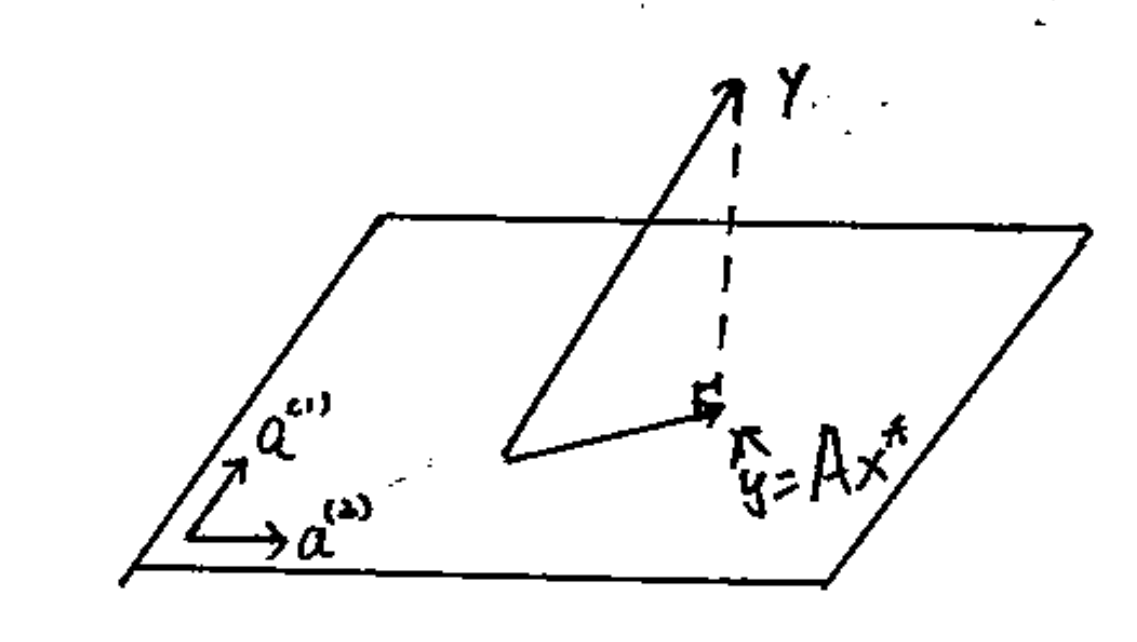
\includegraphics[width=2.1in,height=2.1in]{figures/ch06/figure1.png}
	%\caption{This is an inserted JPG graphic} 
	%\label{fig:graph} 
\end{figure}

From chapter2, 

\begin{equation*}
y^* = \sum^n_{i=1}x_i^*a^{(i)}
\end{equation*}
where 
$$ A =   
\left[
\begin{matrix}
a^{(1)} & ... & a^{(n)}
\end{matrix}
\right]
$$

Solve for $x^*$ via
\begin{equation*}
\sum^n_{i=1}x_i^*<a^{(k)}, a^{(i)}> = <a^{(k)}, y>, \quad \forall k \in \{1,2,...,m \}
\end{equation*}

Stack up to get 
\begin{equation*}
A^TAx^* = A^Ty
\end{equation*}

There are 2 possibilities: (1)$A^TA$ is invertible; (2) $A^TA$ is not invertible.

1) When $A^TA$ is invertible
\begin{align*}
x^* &= (A^TA)^{-1}A^Ty\\
\hat{y}^* &= A(A^TA)^{-1}A^Ty
\end{align*}

2) When $A^TA$ is not invertible
We apply SVD to $A^T A$
\begin{align*}
\hat{y}^* &= A(A^TA)^{-1}A^Ty\\
&= A(V
\begin{bmatrix}
\Sigma & \textbf{0}
\end{bmatrix}
\mathcal{U}^T\mathcal{U}
\begin{bmatrix}
\Sigma \\
\textbf{0}
\end{bmatrix}
V^T)^{-1}A^Ty\\
&= A(V\Sigma^2V^T)^{-1}A^Ty\\
&= AV(\Sigma^{-1})^2V^TA^Ty\\
&= \mathcal{U}
\begin{bmatrix}
\Sigma \\
\textbf{0}
\end{bmatrix}
V^TV\Sigma^{-2}V^TV
\begin{bmatrix}
\Sigma & \textbf{0}
\end{bmatrix}
\mathcal{U}^Ty\\
&= \mathcal{U}
\begin{bmatrix}
\Sigma \\
\textbf{0}
\end{bmatrix}
\Sigma^{-1}\Sigma^{-1}
\begin{bmatrix}
\Sigma & \textbf{0}
\end{bmatrix}
\mathcal{U}^Ty\\
&= \mathcal{U}
\begin{bmatrix}
I_r\\
\textbf{0}
\end{bmatrix}
\begin{bmatrix}
I_r & \textbf{0}
\end{bmatrix}
\mathcal{U}^Ty\\
&= \mathcal{U}
\begin{bmatrix}
I_r& \textbf{0}\\
\textbf{0} & \textbf{0}
\end{bmatrix}
\mathcal{U}^Ty\\
&= \mathcal{U}
\begin{bmatrix}
I_r& \textbf{0}\\
\textbf{0} &  \textbf{0}
\end{bmatrix}
\begin{bmatrix}
<u^{(1)}, y>\\
<u^{(2)}, y>\\
\vdots\\
<u^{(m)}, y>
\end{bmatrix}\\
&= \sum^r_{i=1}<u^{(i)}, y>u^{(i)}
\end{align*}



b) Uniquely determined: ($m =n$)
\begin{equation*}
[A]x = y
\end{equation*}
So,
\begin{equation*}
x^* = A^{-1}y
\end{equation*}

\begin{itemize}
	\item $A$ has full rank (columns\& rows).
	
	\item equal number of constraints and parameters.
	
	\item $A$ is square matrix with full rank so $A^{-1}$ exists.
\end{itemize}

c) Underdetermined($m<n$)

\begin{itemize}
	\item $A$ has full row-rank.
	
	\item $\rank(A) = m$.
	 
	\item $A$ is a wide and short matrix.
	
	\item More parameters than constraints.
	
	\item Hence there are many solutions.
\end{itemize}

Idea: pick solution $x$ that satisfies($*$) with the shortest length in the sense of $L_2$ norm

\begin{equation*}
x^* = \arg \, \min_{Ax = y, x\in \reals^n}\vert x\Vert_2
\end{equation*}

\begin{equation*}
\min_{Ax = y, x\in \reals^n}||x|| = \min_{x\in \reals^n, x\in \mathcal{A}}||x - 0|| = \prod_{\mathcal{A}}(0)
\end{equation*}


\begin{figure}
	\centering
	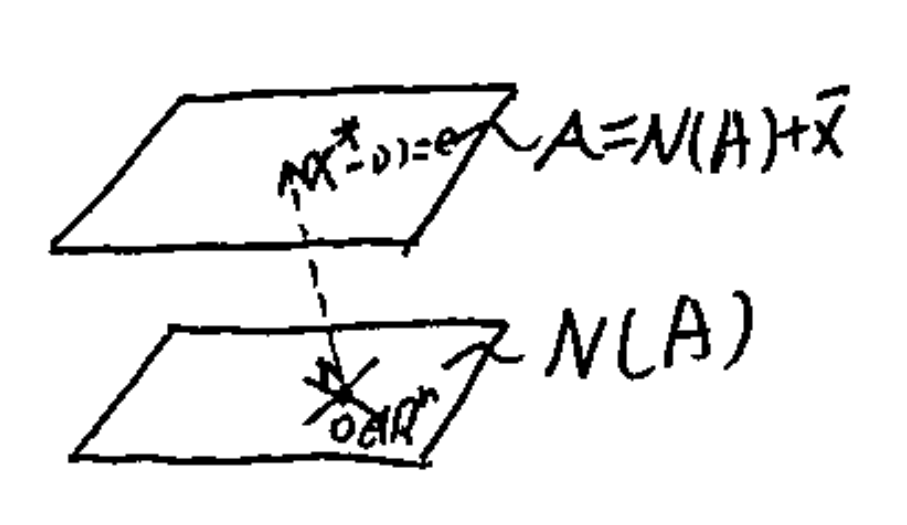
\includegraphics[width=2.1in,height=2.1in]{figures/ch06/figure3.png}
	%\caption{This is an inserted JPG graphic} 
	%\label{fig:graph} 
\end{figure}

To solve for $x^*$, note (from before) error vector 
\begin{align*}
e &= x^* - 0 = x^* \perp N(A)\\
x^* &\in N(A)^{\perp} = R(A^T)
\end{align*}

So we can write $x^* = A^T\alpha$ for some $\alpha \in \reals^m$. 
For $x^*$ to be in $\mathcal{A}$ it must be satisfies that $Ax^* = y$

Substituting in we get 
\begin{equation*}
y = Ax^* = AA^T\alpha
\end{equation*}

By assumption, $A$ is full row rank so $AA^T$ is invertible.
$$x^* = A^T \alpha = A^T(AA^T)^{-1}y$$

Furthermore, we apply SVD to $AA^T$,
\begin{align*}
x^* &= A^T(AA^T)^{-1}y\\
&= A^T\left[\mathcal{U}
\begin{bmatrix}
\Sigma & \mathbf{0}
\end{bmatrix}
V^TV
\begin{bmatrix}
\Sigma\\
\mathbf{0}
\end{bmatrix}
\mathcal{U}^T\right]^{-1}y\\
&= A^T(\mathcal{U}\Sigma^2\mathcal{U}^T)^{-1}y\\
&= A^T\mathcal{U}\Sigma^{-2}\mathcal{U}^Ty\\
&= V
\begin{bmatrix}
\Sigma\\
\mathbf{0}
\end{bmatrix}
\mathcal{U}^T\mathcal{U}\Sigma^{-2}\mathcal{U}^Ty\\
&=V
\begin{bmatrix}
\Sigma^{-1} \\
\mathbf{0}
\end{bmatrix}
\mathcal{U}^Ty\\
&= V
\begin{bmatrix}
\Sigma^{-1}\\
\mathbf{0}
\end{bmatrix}
\begin{bmatrix}
<u^{(1)}, y>\\
...\\
<u^{(n)}, y>
\end{bmatrix}\\
&= \sum^r_{i=1}\frac{1}{\sigma_i}<u^{(i)}, y>v^{(i)}
\end{align*}




%last time

%solving linear system of equations Ax=y

%1. over determined
%
%$A^TAx=A^Ty$


%2. under determined m<n

%$X^* \in R(A^T)  $ 

%3. invertiable





\subsection{Interpretation of $x^*= \arg \min_x \Vert y-Ax\Vert_2$}

\quad\ (1). Approximated solution to $y=Ax$

$y^*=Ax^*$ is the 'best' approximated solution in the sense of $L_2$ norm, which means, $y^*$ is the closest point in $R(A)$ to $y$.

(2). Minimum perturbation of $y$ to 'feasibility'

\begin{figure}
	\centering
	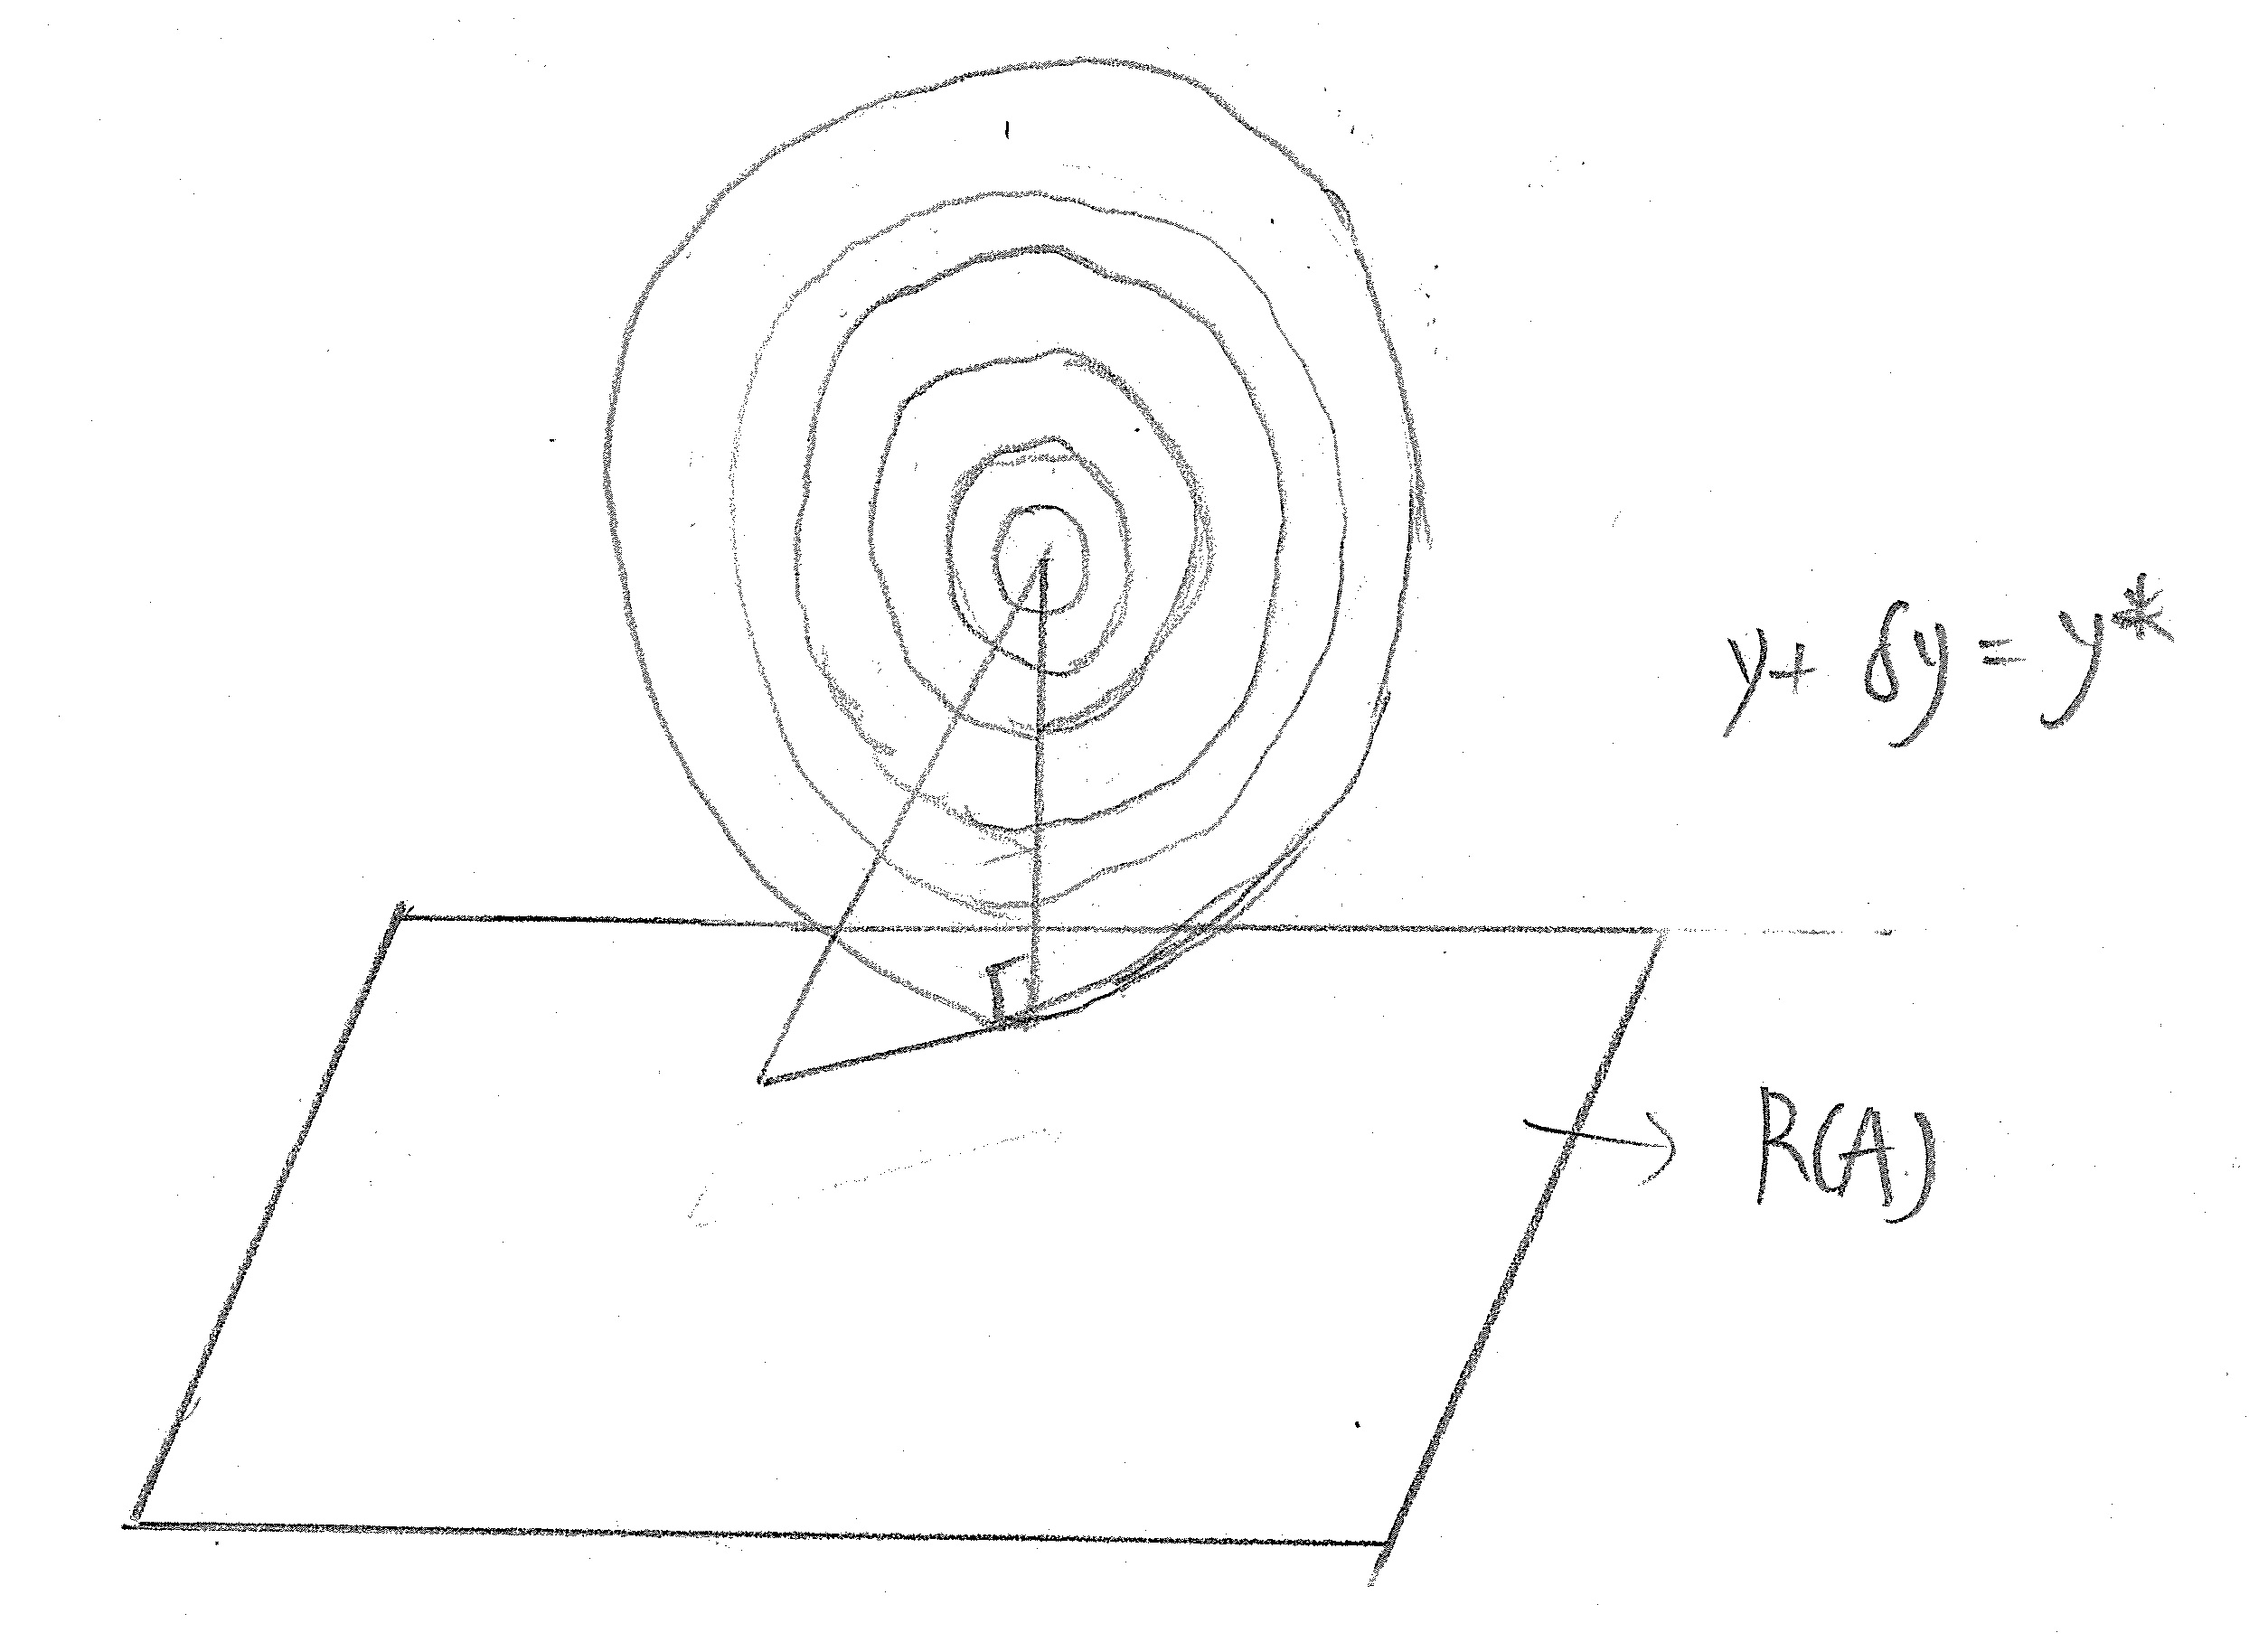
\includegraphics[width=2in,height=2in]{figures/ch06/ch06-01.jpg}
	%\caption{This is an inserted JPG graphic} 
	%\label{fig:graph} 
\end{figure}

(3). Perturb both $y$ and $A$ to get 'feasibility'

'Total least square'
$$\min_{\delta y,  \delta A} \Vert [\delta A\  \delta y] \Vert_F$$

where $\delta A$ is $m$ by $n$ matrix and thus $[\delta A\  \delta y]$ is $m$ by $n+1$, $y+\delta y\in R(A+\delta A)$.


(4). Linear regression
$$\Vert y-Ax\Vert ^2_2 = \sum_{i=1}^{m} ( y_i - <a^{(i)} , x>)^2 = \sum_{i=1}^{m} r_i^2$$
where $r_i$ defined as the residual.

\begin{figure}
	\centering
	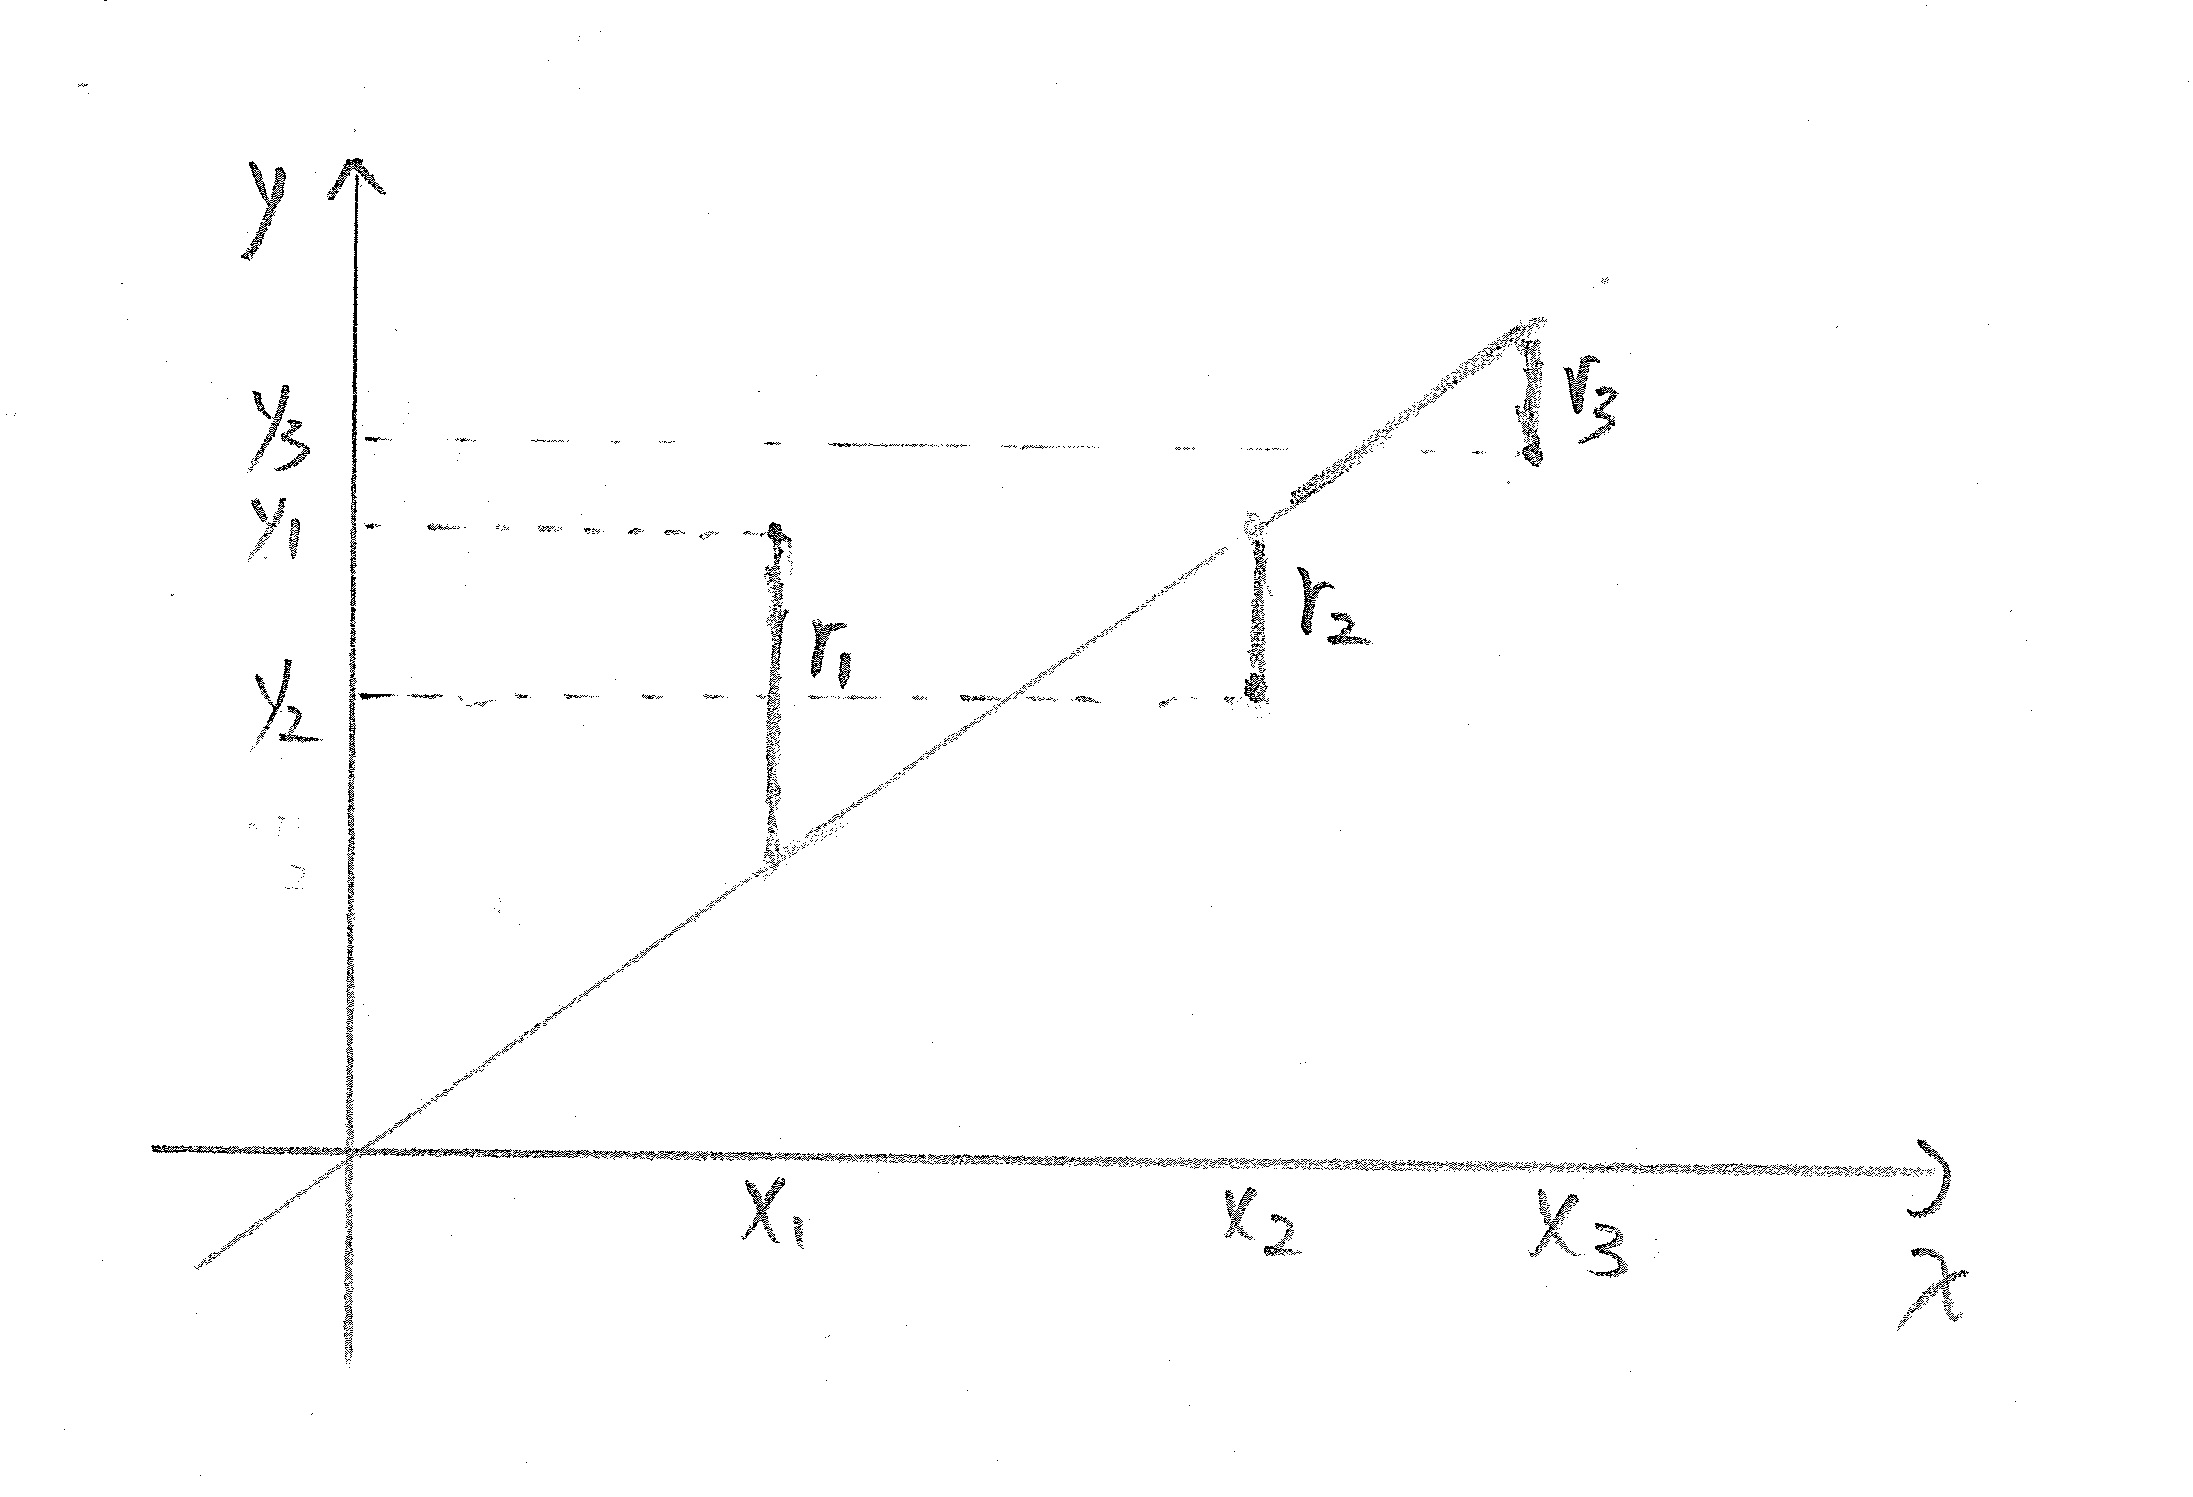
\includegraphics[width=2in,height=2in]{figures/ch06/ch06-02.jpg}
	%\caption{This is an inserted JPG graphic} 
	%\label{fig:graph} 
\end{figure}



\vspace{0.5cm}
Example

Let's consider fitting a line to $\{(0,6),(1,0),(2,0) \}={(a_i,y_i)}.$

The approximation takes the form of $y=x_1+ax_2$, and we want to choose a vector x to minimize $\sum_{i=1}[y_i-(x_1+a_ix_2)]^2 = \sum_{i=1} r_i^2$,

\begin{align*}
\Vert y- Ax\Vert_2^2 
&=
\left\Vert
\begin{bmatrix}
6\\
0\\
0
\end{bmatrix}
-
\begin{bmatrix}
1&0\\
1&1\\
1&2
\end{bmatrix}
\begin{bmatrix}
x_1\\
x_2
\end{bmatrix}
\right\Vert_2^2\\
&=\Vert y-Ax^*\Vert^2_2\\
&=6
\end{align*}

Solve for $x^*$, we have
$x^*=(A^TA)^{-1}A^Ty=[5 , -3]^T$

Thus, the equation for this line is
$$\hat{y}=x_1^*+ax_2^*=5-3a$$            %so x1 and x2 are parameters




\subsection{Variants of least square}

In the previous classical least square method, we do not consider the weights for each square of the residual(i.e., all of them are equally weighted), however, some residuals might be more important than the others. A very natural approach is to assign different weights to different $r_i^2$.

\vspace{0.3cm}
Weighted least square:
\begin{align*}
\min \sum_{i=1}^{n} w_i^2 r_i^2
&=\Vert W (y-Ax)\Vert ^2_2\\
&=\Vert Wy-WAx)\Vert ^2_2\\
&=\Vert \bar{y}-\bar{A}x \Vert ^2_2
\end{align*}

where $W=\diag(w_1, w_2, \cdots, w_m)$ and each $w_i\geq 0$, $\bar{y} \triangleq Wy$ and $\bar{A} \triangleq WA$. From the last two equities, we may find that this is very similar with the classic one but now we need to solve for $x$ in a transformed coordinate system.

In fact, we can use a more general transform with PSD:
$$\Vert W (y-Ax)\Vert ^2_2 = (y-Ax)^TW^TW(y-Ax)=r^TW^TWr$$
Note that $r$ is the residual in the original coordinate system. Solve for $x^*$, we have 
$$x^*=(A^T W W^T A)^{-1} A^T W W^T y$$

\vspace{0.3cm}
Standard LS
\begin{figure}
	\centering
	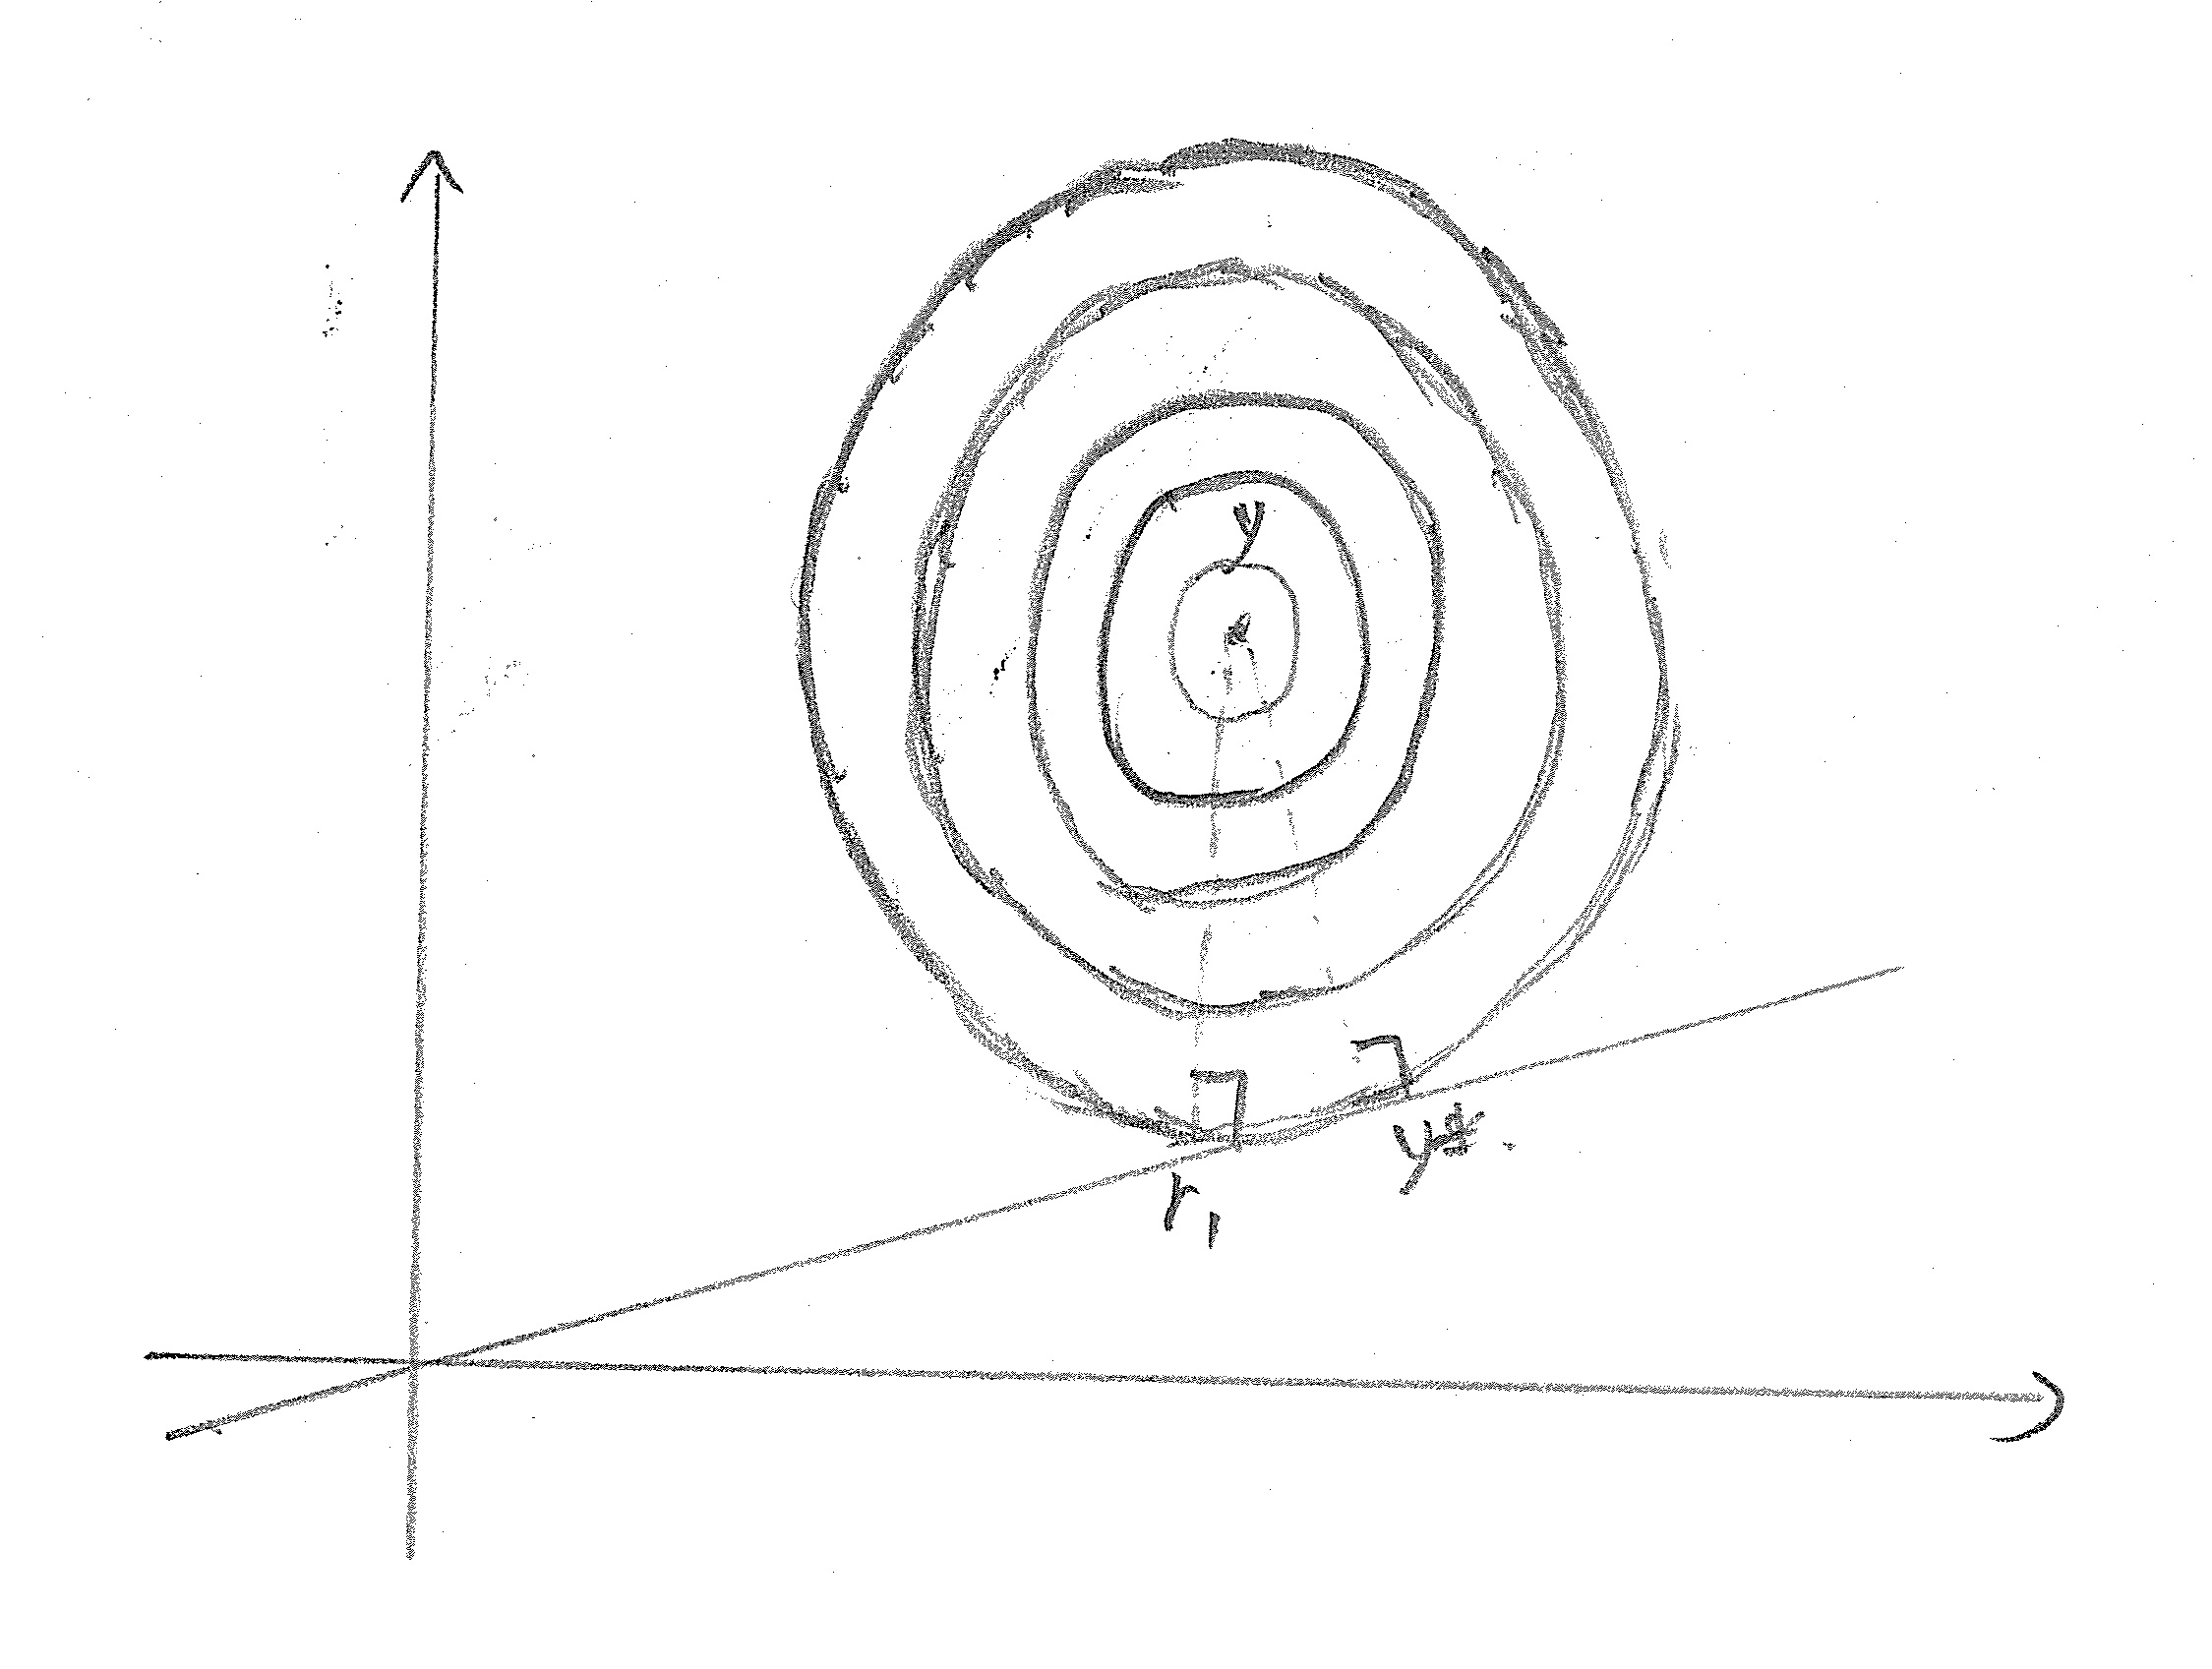
\includegraphics[width=2in,height=2in]{figures/ch06/ch06-03.jpg}
	%\caption{This is an inserted JPG graphic} 
	%\label{fig:graph} 
\end{figure}

Weighted LS with $W$ is diagonal 

\begin{figure}
	\centering
	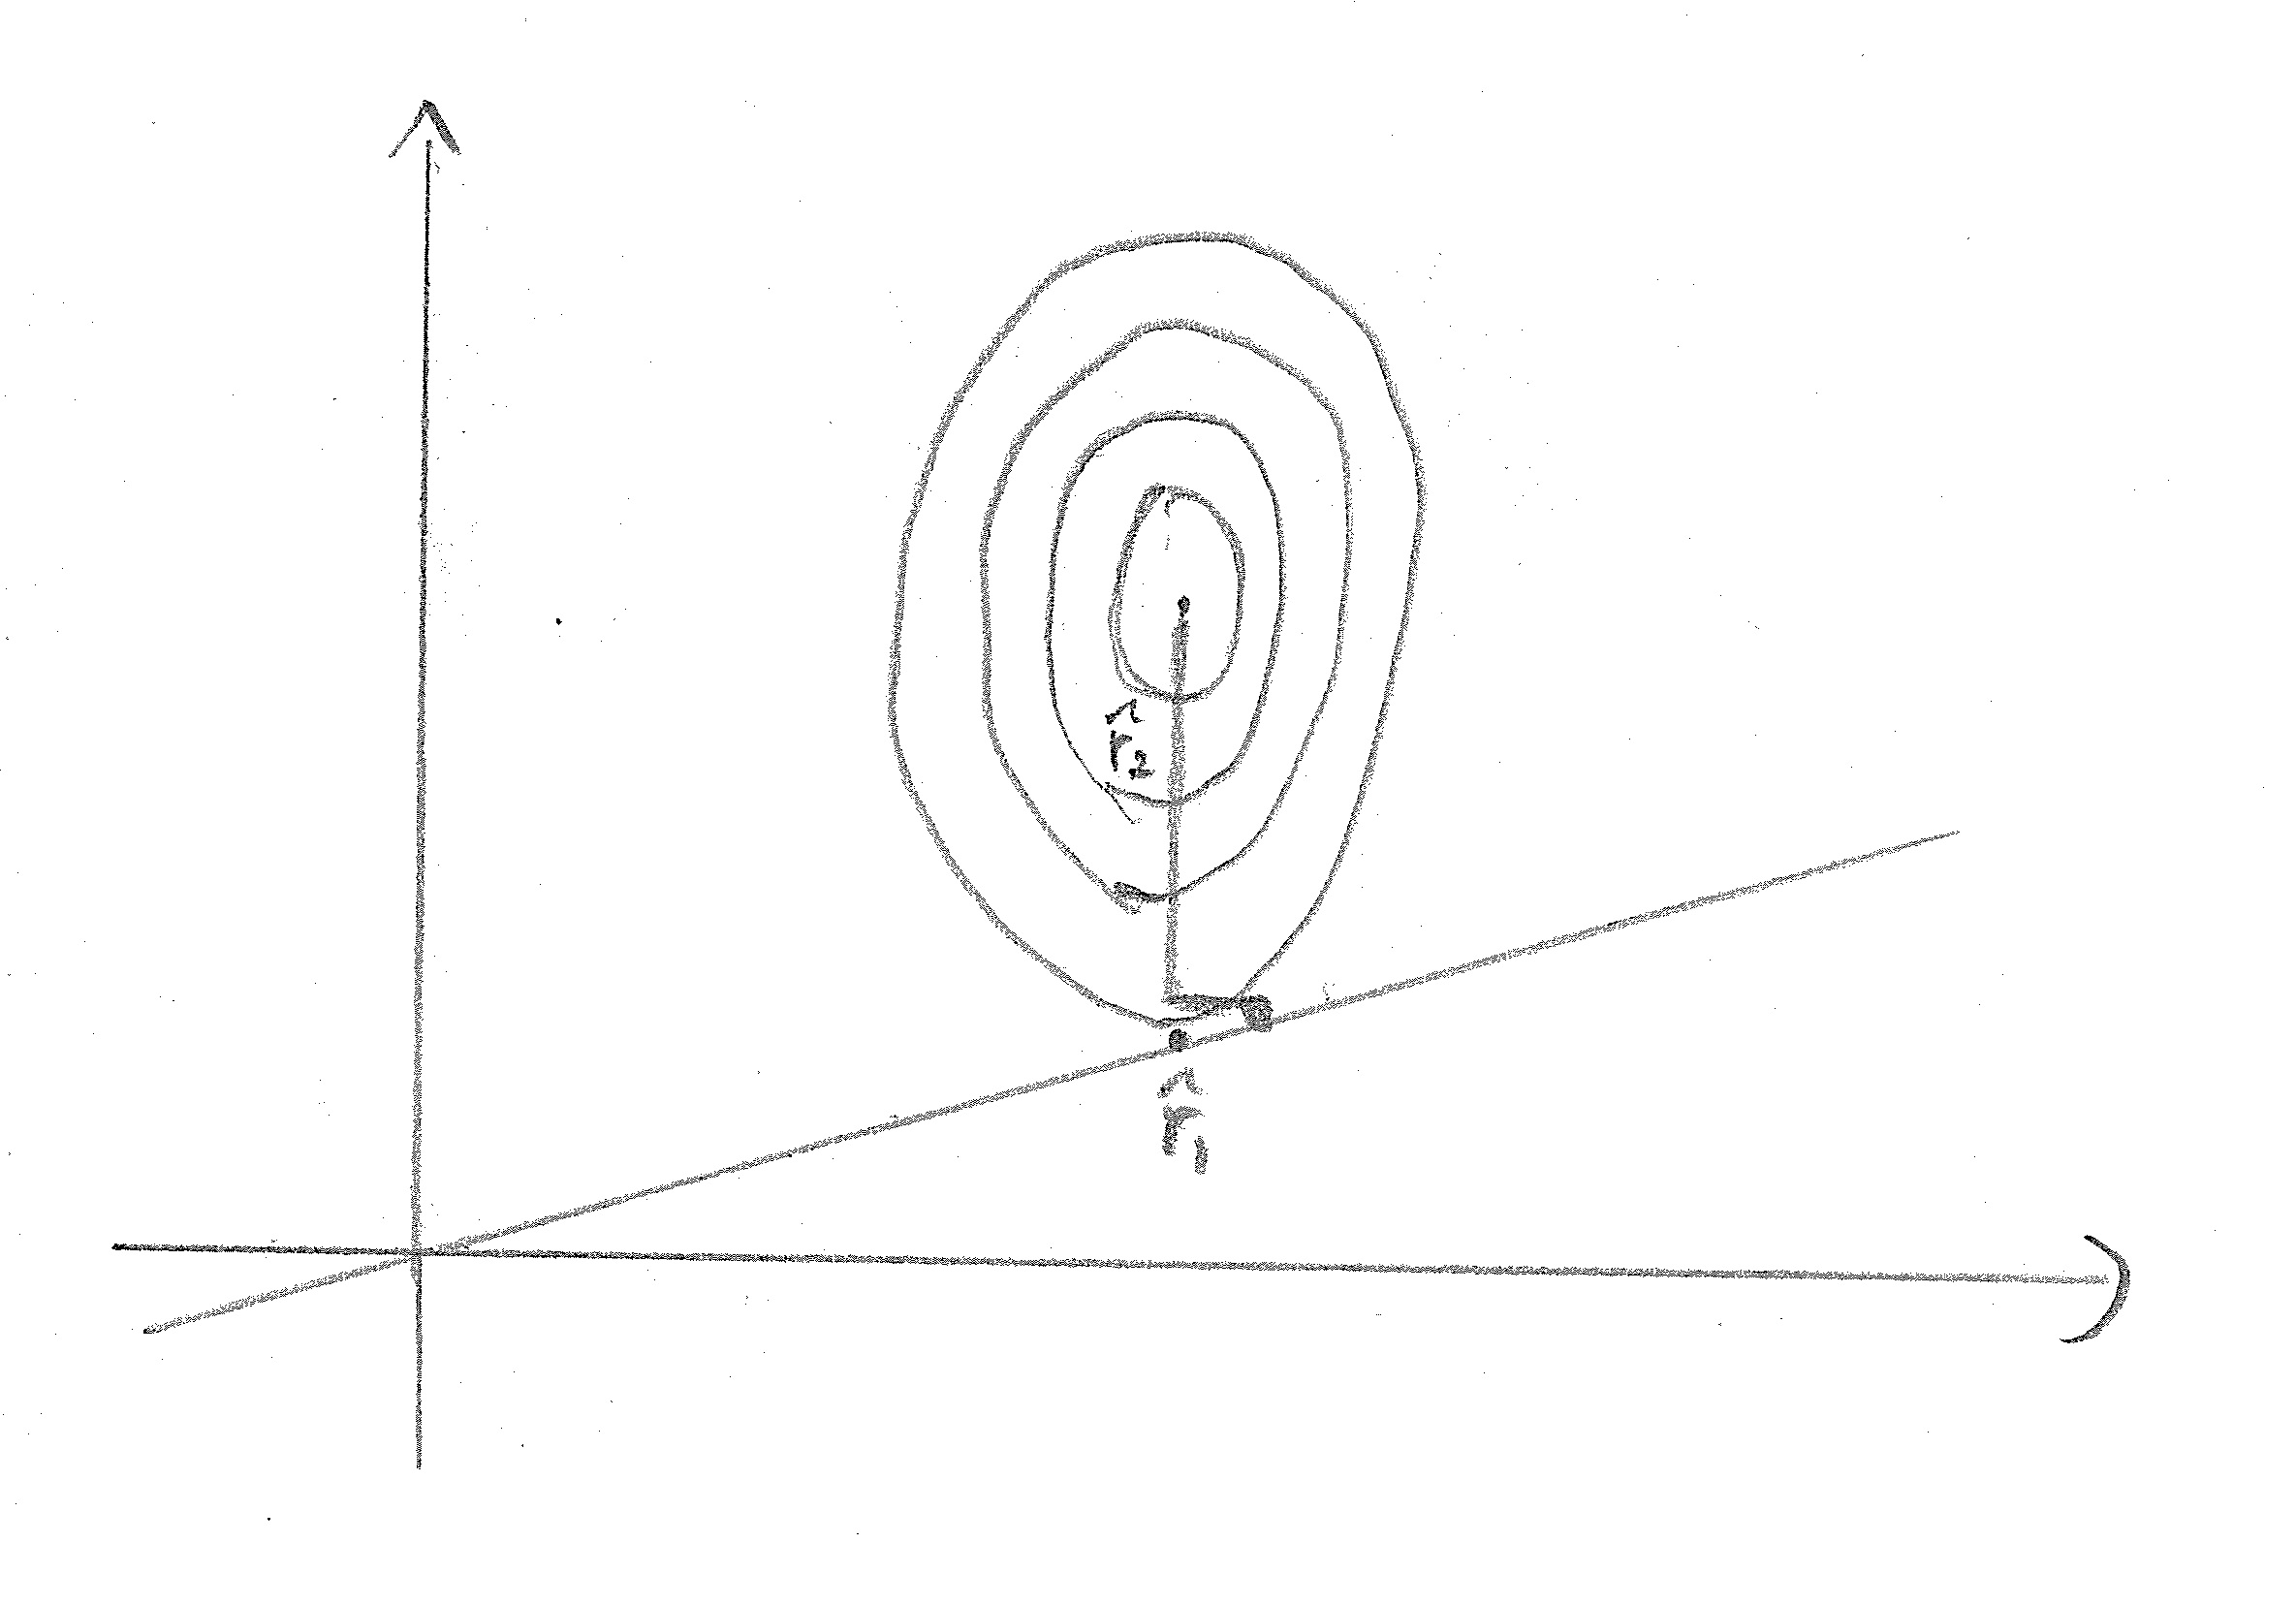
\includegraphics[width=2in,height=2in]{figures/ch06/ch06-04.jpg}
	%\caption{This is an inserted JPG graphic} 
	%\label{fig:graph} 
\end{figure}

Weighted LS with $W$ is PSD (rotation)

\begin{figure}
	\centering
	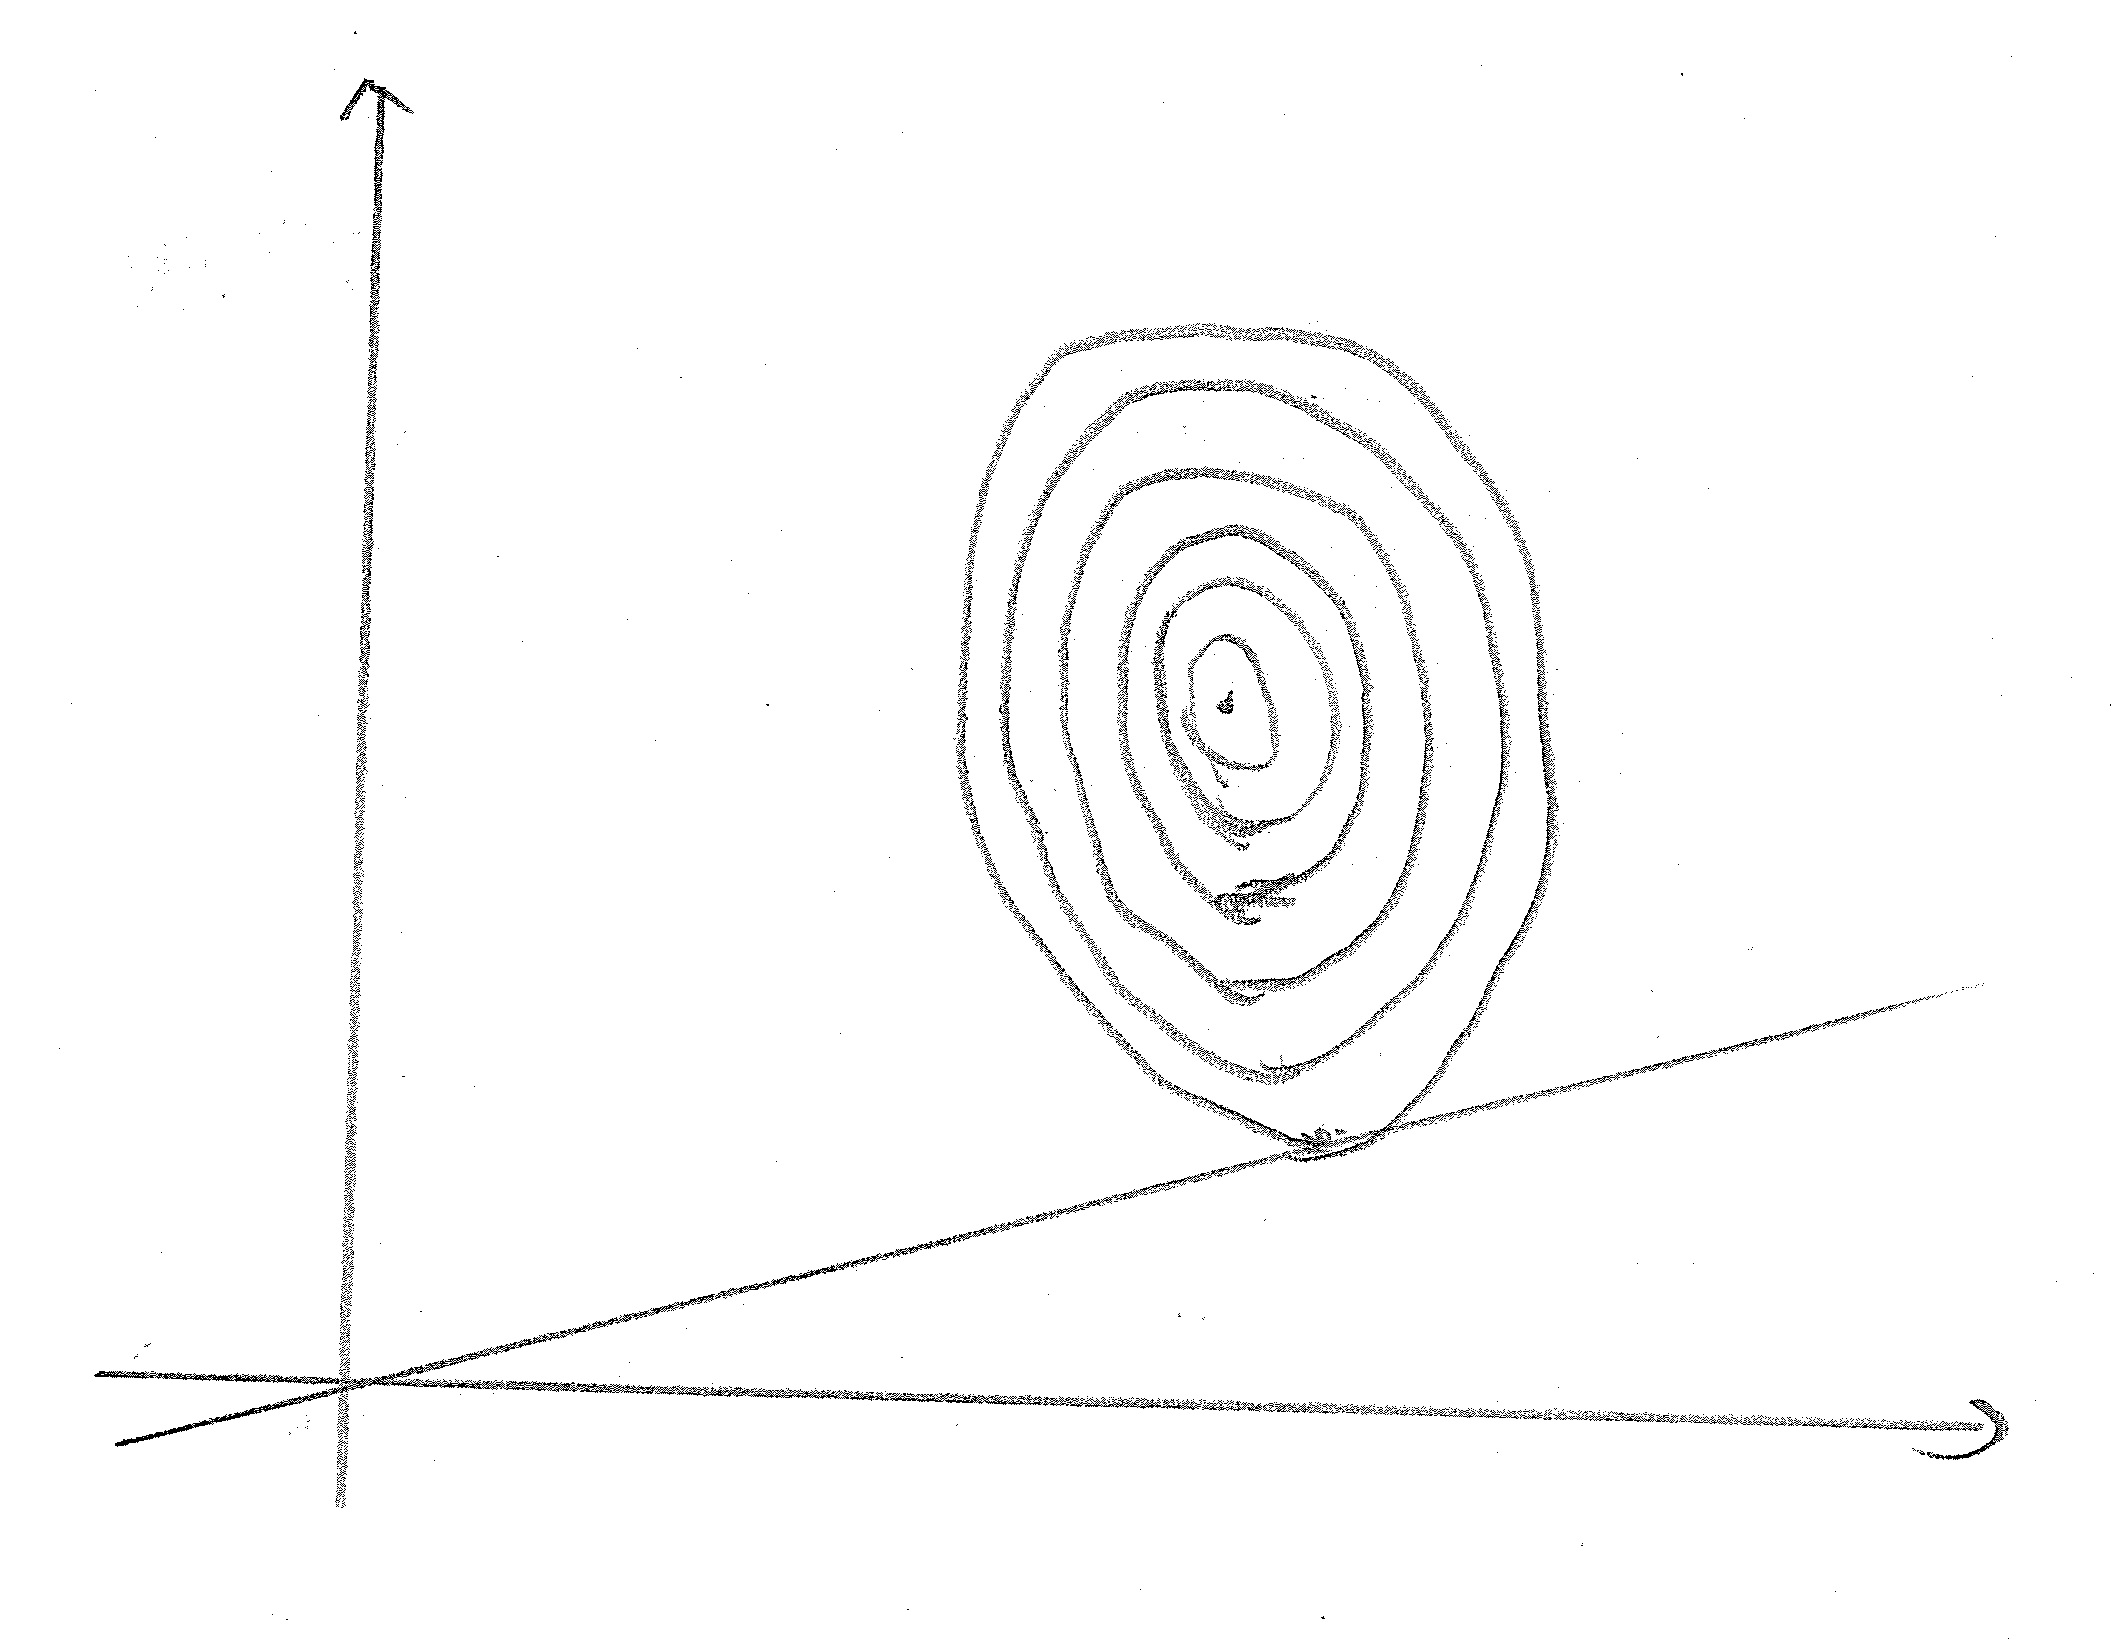
\includegraphics[width=2in,height=2in]{figures/ch06/ch06-05.jpg}
	%\caption{This is an inserted JPG graphic} 
	%\label{fig:graph} 
\end{figure}



\subsection{$L_2$- regularization least square}


In the original least square, 
$$x*=\arg_{x\in\reals_{n}} \min \Vert Y-Ax\Vert ^2_2$$

we do not have preference for any specific $x$ over any other, and often $x$ is a vector of resources consumed.


Regularized least square
$$x^*=\arg_{x\in\reals_{n}} \min \Vert y-Ax\Vert ^2_2 + \gamma \Vert x\Vert ^2_2$$
where $\gamma$ is a non negative scalar(so if $\gamma = 0$ we retrieve the original LS)


To solve regularized least square, first note that if we have
$$u\in\reals^{n}, v\in\reals^{m}$$

We can define 
$$
\bar{A}=
\begin{bmatrix}
A\\
\gamma I
\end{bmatrix}
,
\bar{y}=
\begin{bmatrix}
y\\
0_n
\end{bmatrix}
$$


$$\Vert Ax - y\Vert ^2_2 + \gamma \Vert x\Vert ^2_2=\Vert \bar{A}x-\bar{y}\Vert^2_2$$

$$x^*=(\bar{A}^T A)^{-1} \bar{A}^T \bar{y}=(A^T A+\gamma I)^{-1} A^T y$$


\vspace{0.5cm}
'Tikhonov' regularization (also known as ridge regression)
$$\min_x \Vert W_1 (Ax - y)\Vert^2_2 - \Vert W_2 (x - x^{(0)})\Vert^2_2 = \min_x \Vert \bar{A}x-\bar{y}\Vert^2_2 $$
where $\bar{A} = 
\begin{bmatrix}
W_1 A\\
W_2
\end{bmatrix}
,
\bar{y} = 
\begin{bmatrix}
	W_1 y\\
	W_2 x^{(0)}
\end{bmatrix}
$
, and $W_1$ and $W_2$ are PSD.


\vspace{0.8cm}
Visualize regularized LS: $\min \Vert Ax-y\Vert_2^2 +\gamma \Vert x\Vert^2_2$

Recall our previous example, 
$$x^*= \arg_{x\in \reals^n} \min =
\left\Vert
\begin{bmatrix}
6\\
0\\
0
\end{bmatrix}
-
\begin{bmatrix}
1&0\\
1&1\\
1&2
\end{bmatrix}
\begin{bmatrix}
x_1\\
x_2
\end{bmatrix}
\right\Vert^2_2
=
\begin{bmatrix}
5\\
-3
\end{bmatrix}
$$
and $\Vert Ax^*-y\Vert_2^2 = 6$.


\begin{figure}
	\centering
	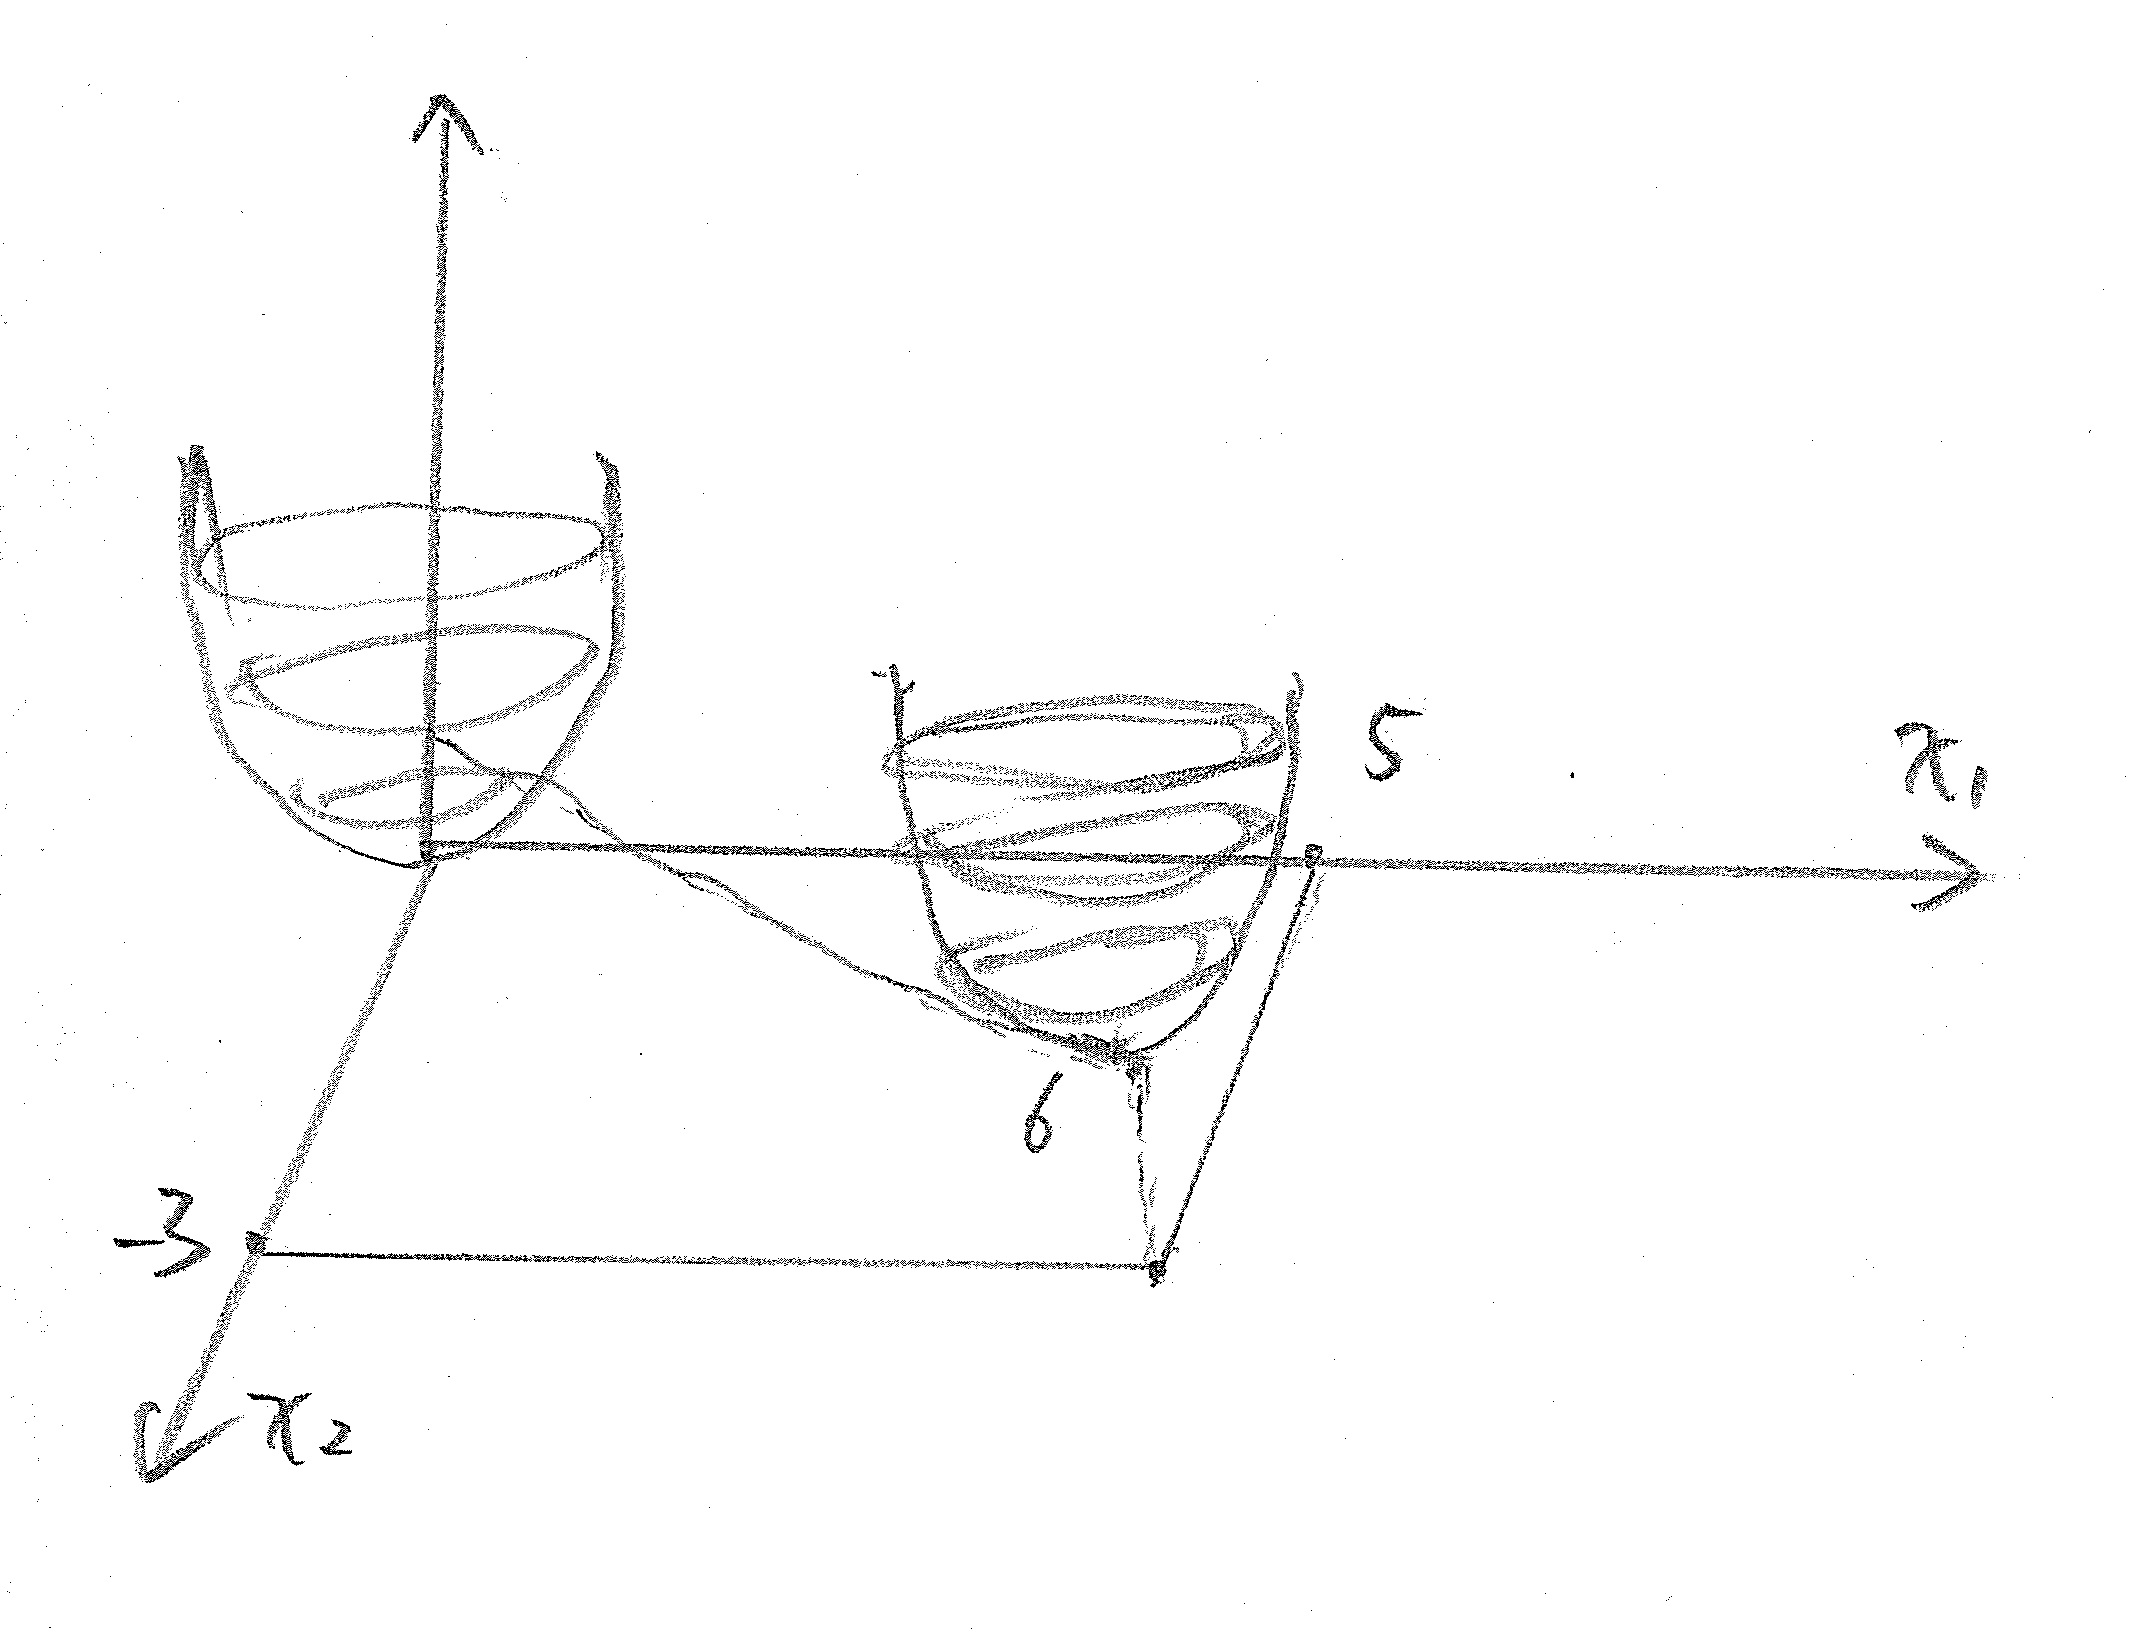
\includegraphics[width=1.8in,height=1.8in]{figures/ch06/ch06-06.jpg}
	%\caption{This is an inserted JPG graphic} 
	%\label{fig:graph} 
\end{figure}

\newpage
Draw level set for same picture
\begin{figure}
	\centering
	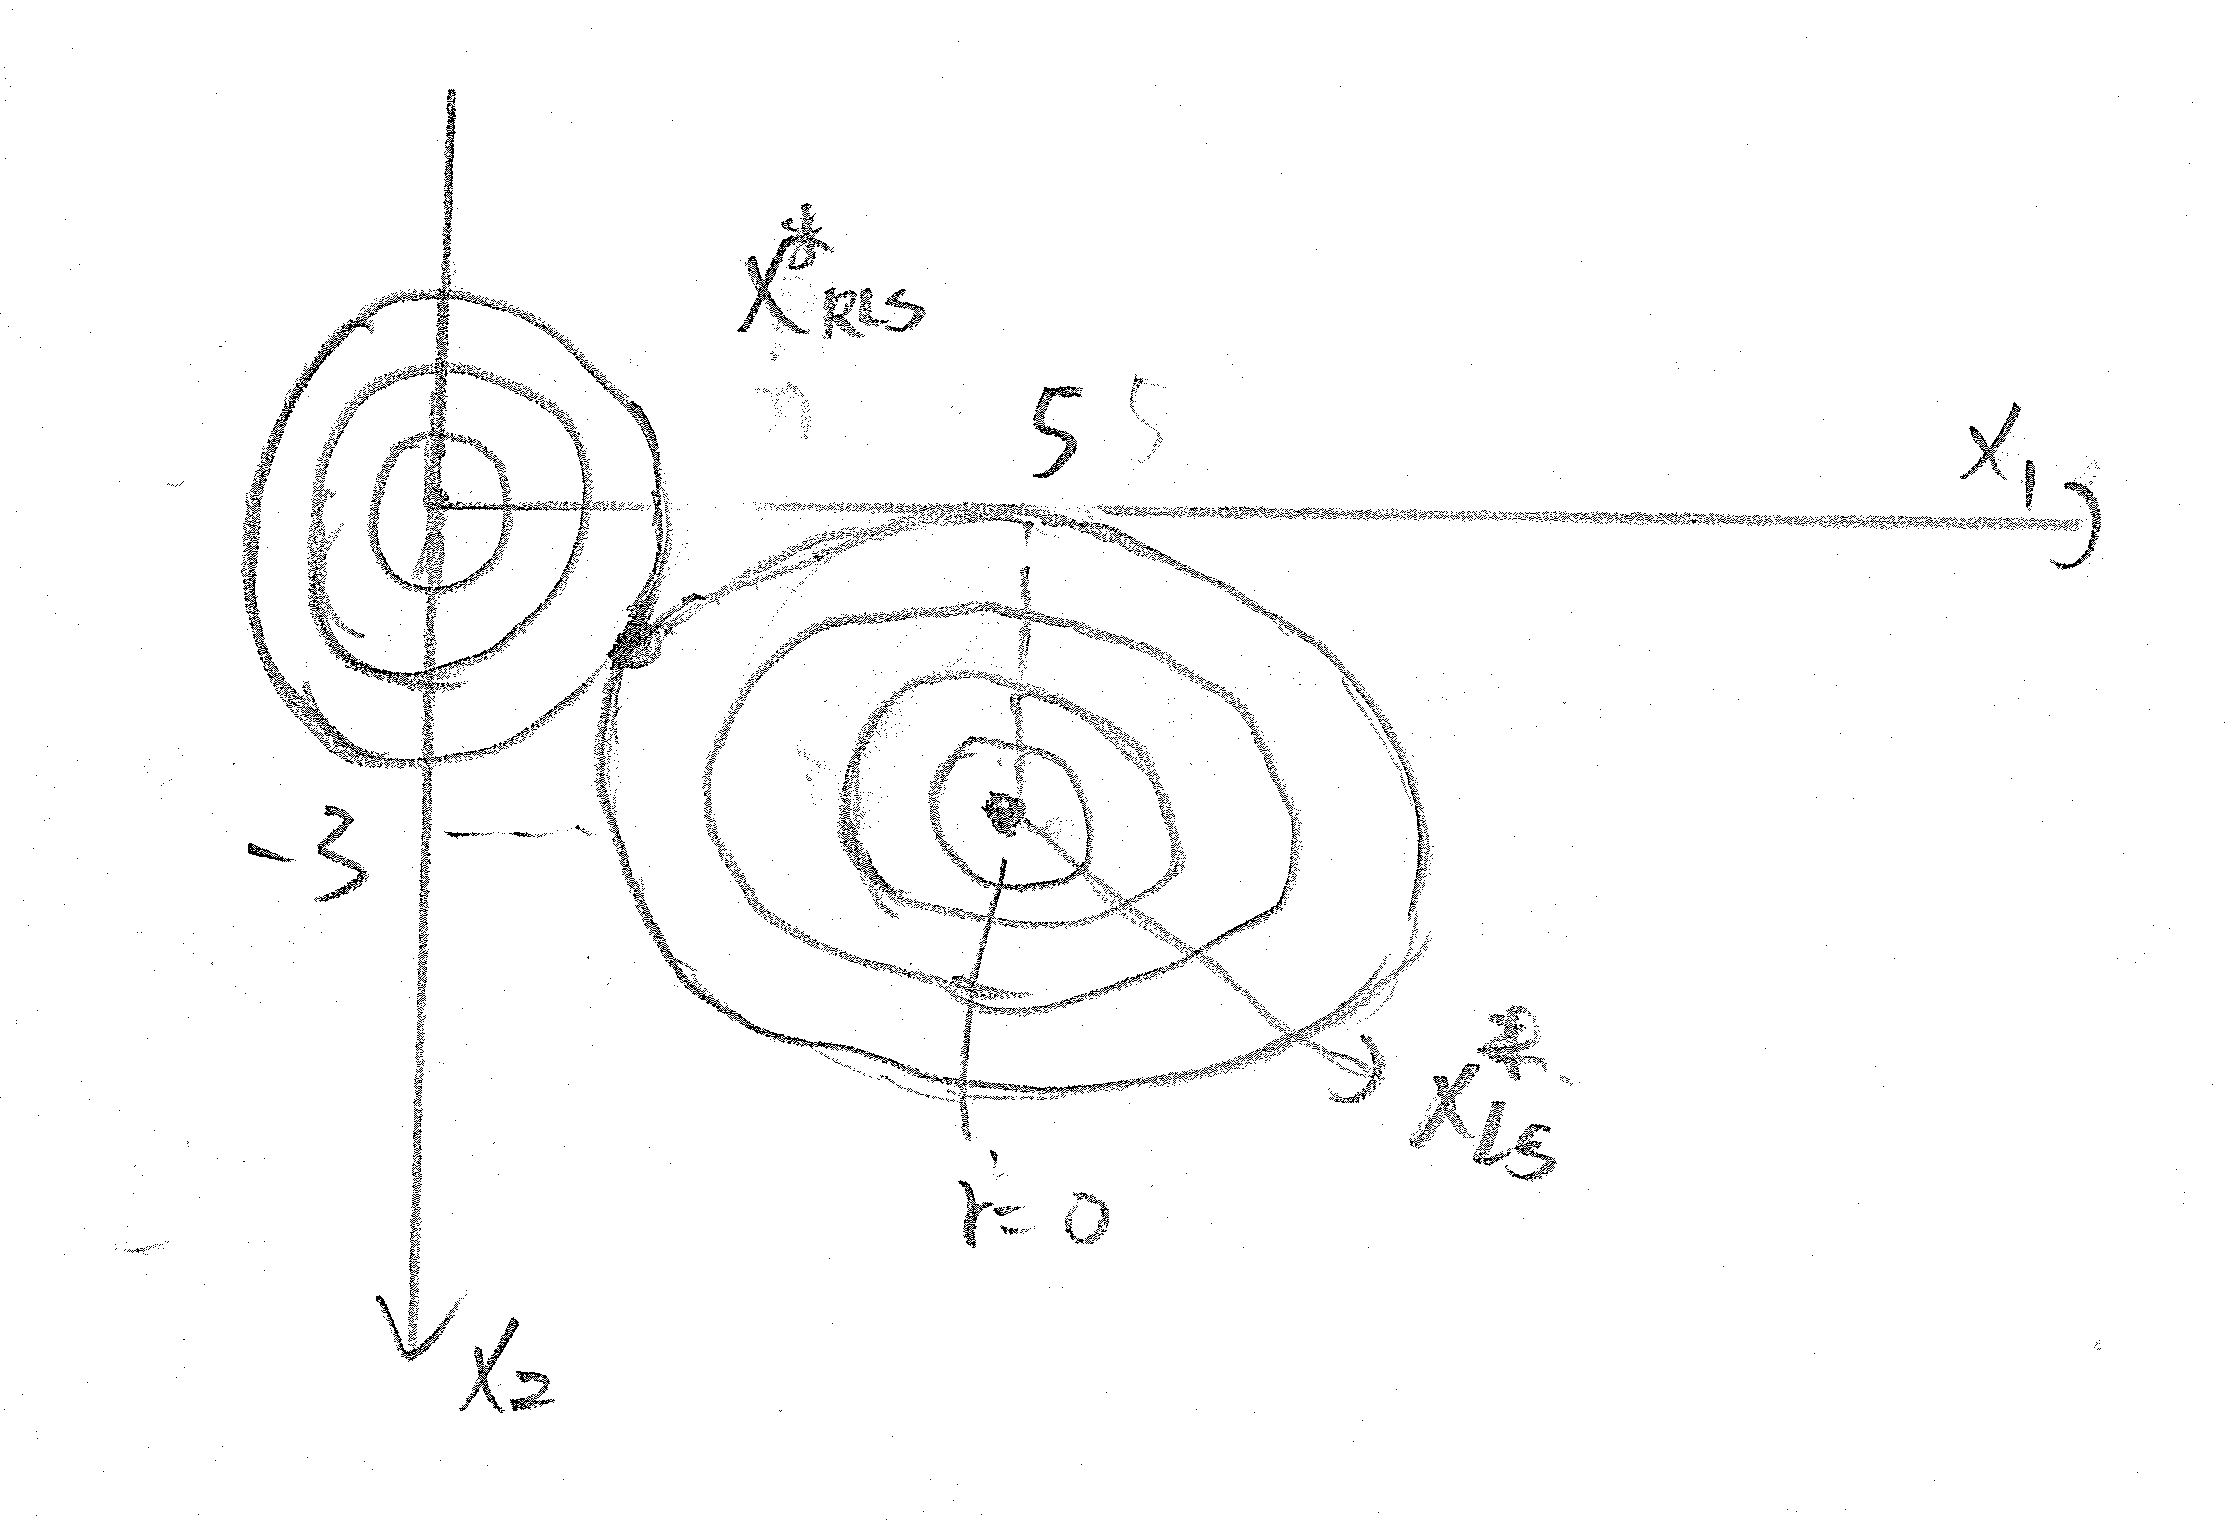
\includegraphics[width=1.8in,height=1.8in]{figures/ch06/ch06-07.jpg}
	%\caption{This is an inserted JPG graphic} 
	%\label{fig:graph} 
\end{figure}

\begin{align*}
c_1
&=\Vert Ax-y\Vert^2_2\\
&=\Vert A(x-x_{ls}^*+x_{ls}^*)-y\Vert^2_2\\
&=\Vert (Ax_{ls}^*-y)-A(x-x_{ls}^*)\Vert^2_2\\
&=\Vert (Ax_{ls}^*-y)\Vert^2_2 - \Vert A(x-x_{ls}^*)\Vert^2_2
\end{align*}

The first term on the last equality is a scalar 6(from previous example), and so we focus on the geometry of second term.
$$\Vert A(x-x_{ls}^*)\Vert^2_2= (x-x_{ls}^*)^T A^TA (x-x_{ls}^*)$$. 
Note that $A^TA$ is a PSD matrix. Understand geometry of level set of $\Vert A(x-x_{ls})\Vert^2_2$ via eigenvector of the PSD matrix $A^T A$

$$A^TA=
\begin{bmatrix}
3&3\\
3&5
\end{bmatrix}
=
\begin{bmatrix}
-0.81&0.58\\
058&0.81
\end{bmatrix}
\begin{bmatrix}
0.84&0\\
0&7.14
\end{bmatrix}
\begin{bmatrix}
-0.81&0.58\\
058&0.81
\end{bmatrix}
$$
\begin{marginfigure}
	\centering
	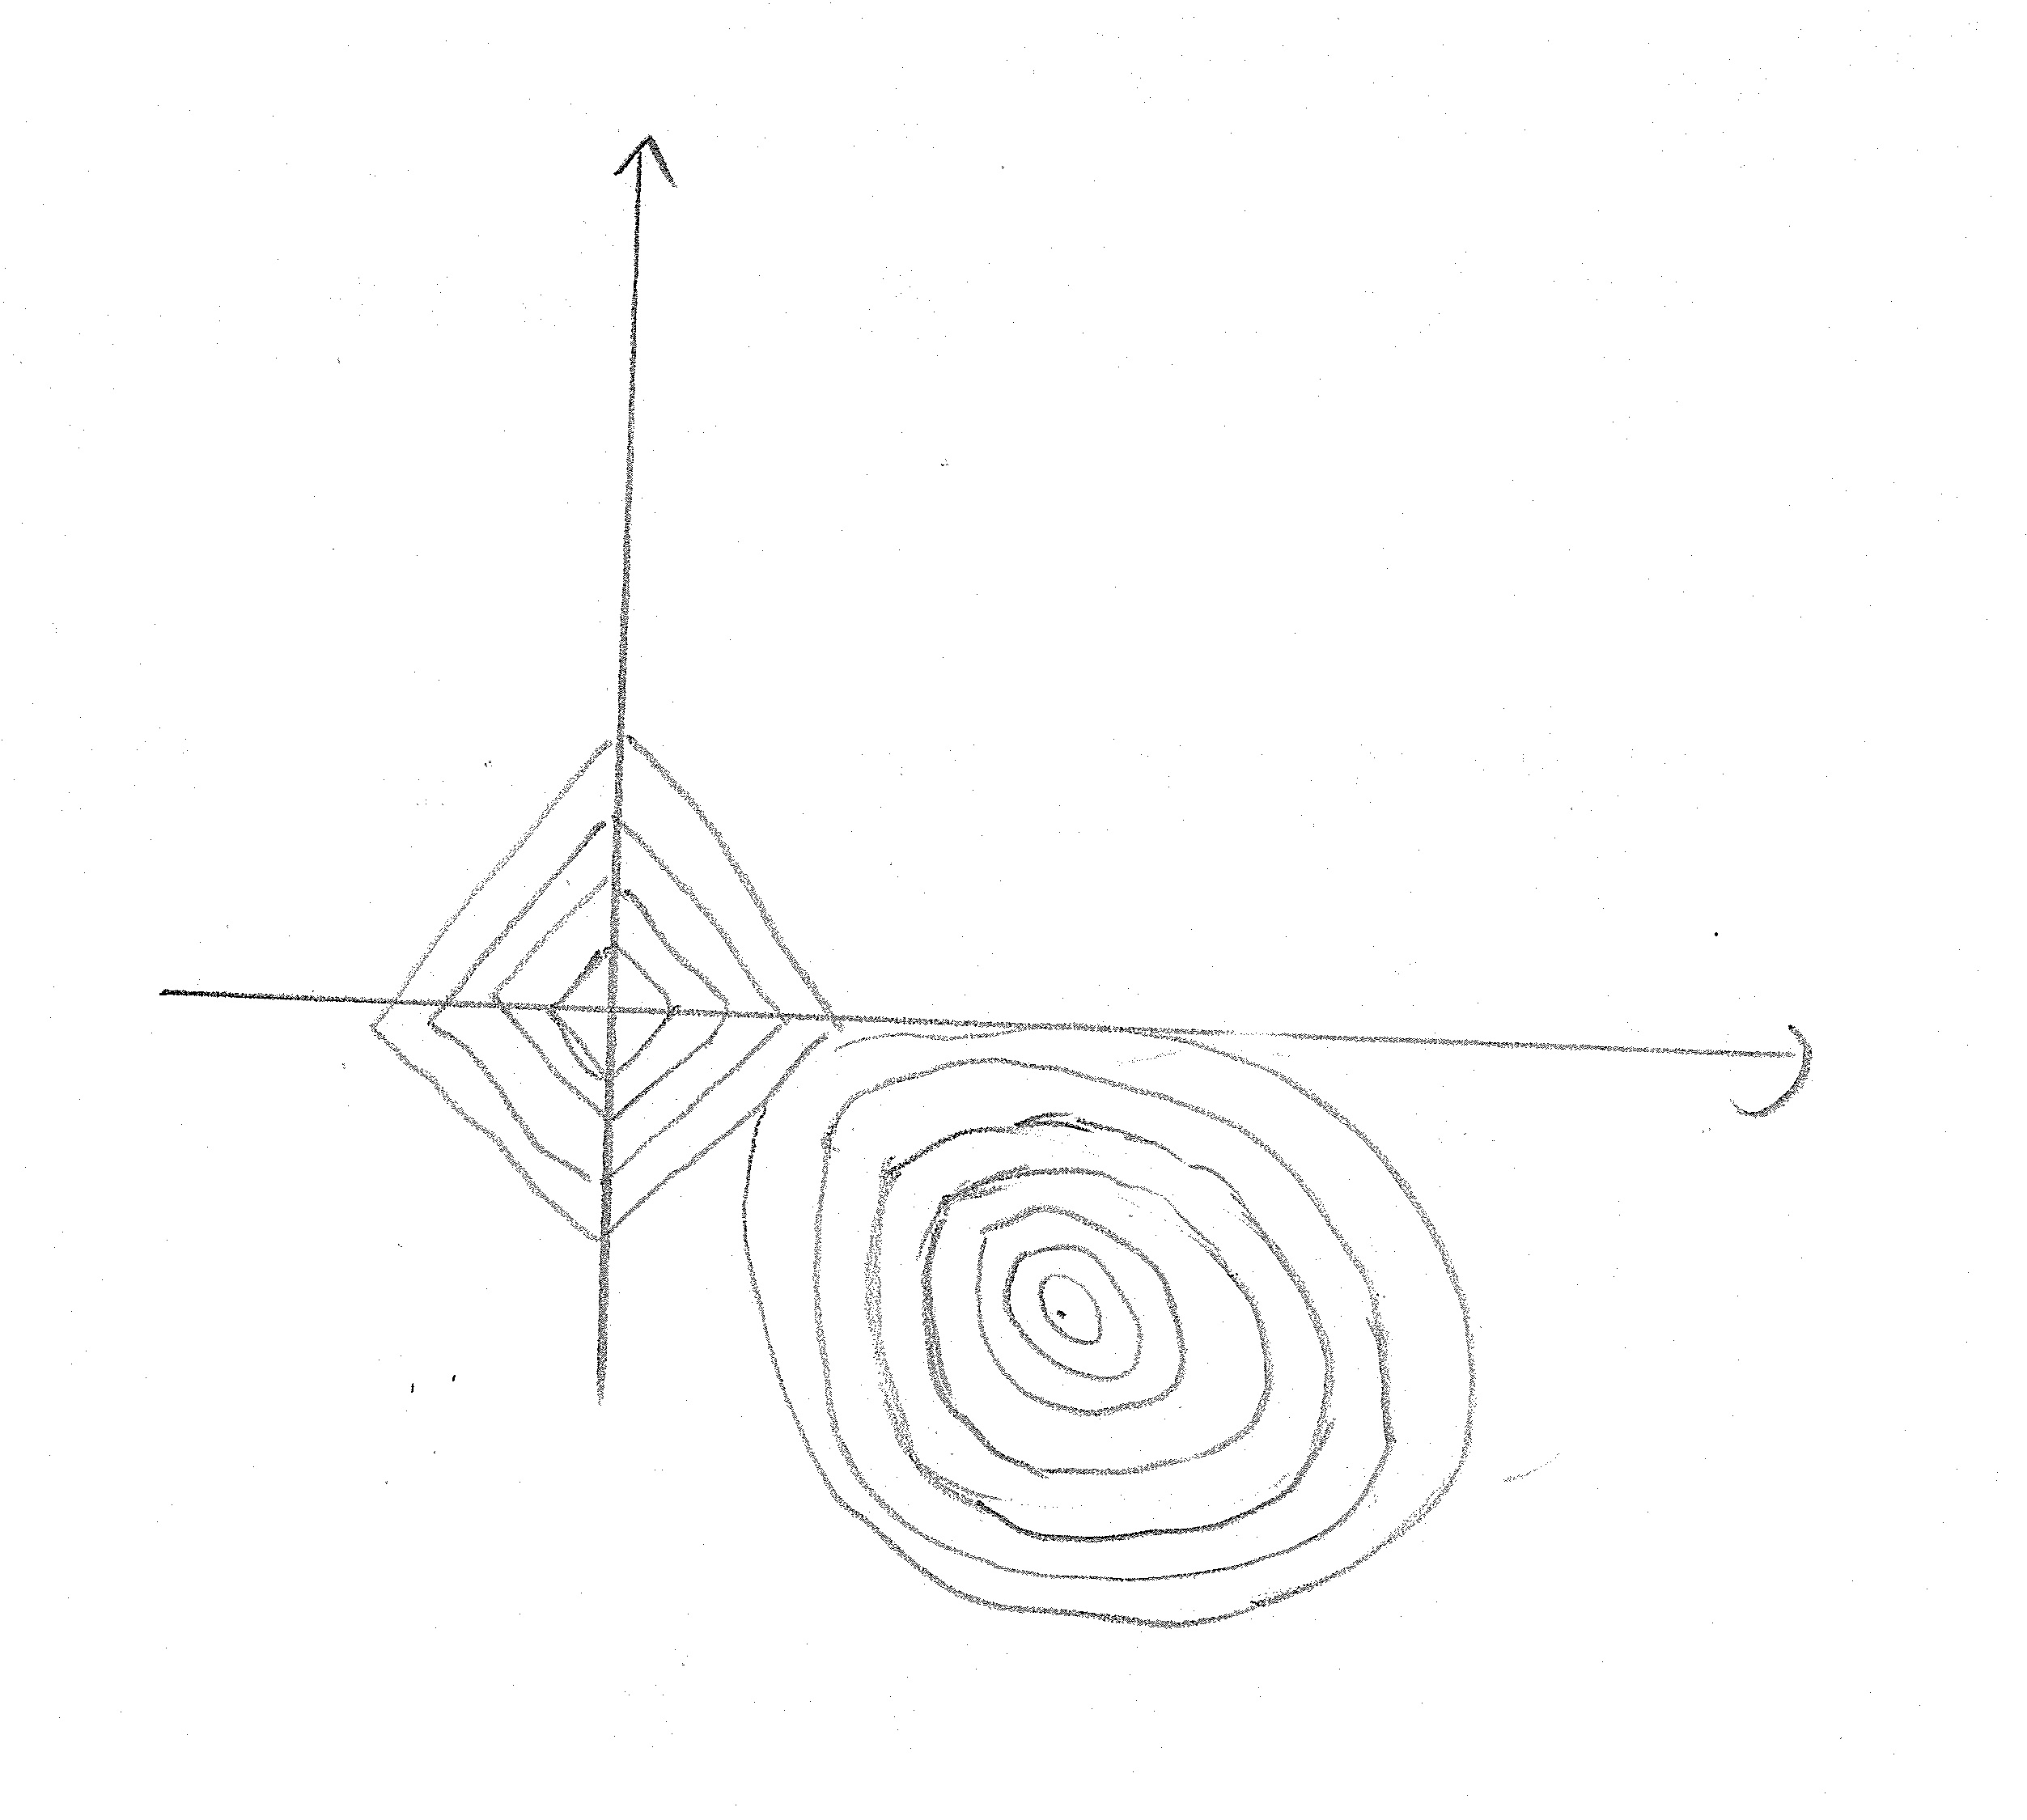
\includegraphics[width=1.8in,height=1.8in]{figures/ch06/ch06-08.jpg}
	%\caption{This is an inserted JPG graphic} 
	%\label{fig:graph} 
\end{marginfigure}


\subsection{Brief summary of Least Squares}
\begin{equation*}
x^* = \arg\, \min_{x\in \reals^n}||y-Ax||_2^2 \,\,\,\,\, (*)
\end{equation*}

	(1) Standard LS variant in ($*$) weights all elements of error vector equally.(weighted LS)
	
	(2) Standard LS measures error along standard coordinate system.(change coordinate system)
	
	(3) Standard LS ignores that certain elements of $x$ may "cost" more than others.(regularization)

\subsection{"Tikhanov regularization"}
$$x^* =arg\,min_{x\in \reals^n}||w_1(y-Ax)||_2^2 + ||w_2(x - x^{(0)})||_2^2$$

We do a simple example:
\begin{equation*}
x^* = arg\,min_{x\in \reals^n}||y-Ax||_2^2 + \gamma||x||_2^2
\end{equation*}

\begin{marginfigure}
	\centering
	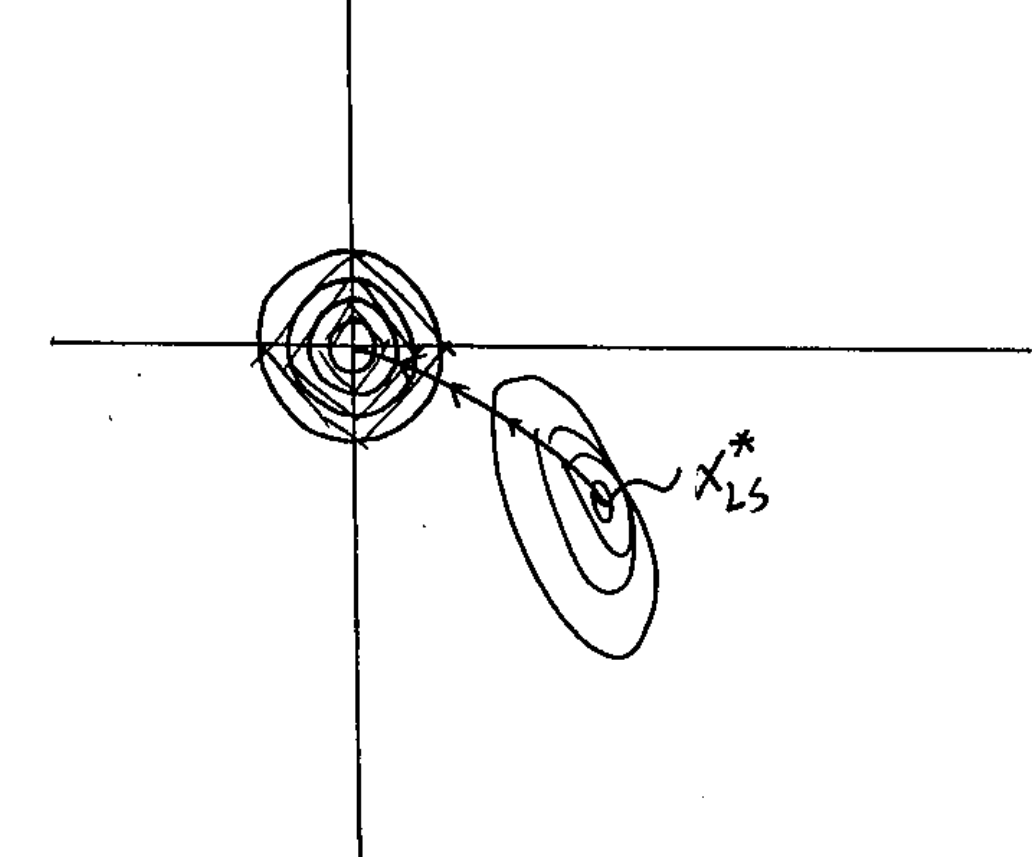
\includegraphics[width=1.8in,height=1.8in]{figures/ch06/figure4.png}
	%\caption{This is an inserted JPG graphic} 
	%\label{fig:graph} 
\end{marginfigure}

Look at form of optional solution to 
\begin{align*}
x^* &= arg\,min_{x\in \reals^n}||y-Ax||_2^2 + \gamma||x||^2_2\\
&= (A^TA + \gamma I)^{-1}A^Ty\\
\hat{y}&= Ax^* = A(A^TA + \gamma I)^{-1}A^Ty\\
\end{align*}
Apply SVD to A,
$$A = \mathcal{U}\tilde{\Sigma}V^T$$

First thing is to analyze $(A^TA + \gamma I)^{-1}$:
\begin{align*}
(A^TA + \gamma I)^{-1} &= (V\tilde{\Sigma}^T\mathcal{U}^T\mathcal{U}\tilde{\Sigma}V^T + \gamma I)^{-1}\\
&= (V
\begin{bmatrix}
\Sigma^T & 0\\
0 & 0\\
\end{bmatrix}
\begin{bmatrix}
\Sigma & 0\\
0 & 0\\
\end{bmatrix}
V^T + \gamma I)^{-1}\\
&=(V
\begin{bmatrix}
\Sigma^2 & 0\\
0  & 0
\end{bmatrix}
V^T + \gamma VV^T
)^{-1}\\
&= (V(
\begin{bmatrix}
\Sigma^2 & 0\\
0 & 0
\end{bmatrix}
+\gamma I)V^T)^{-1}\\
&= V
\left[
\begin{array}{c|c}
\Sigma^2+\gamma I_r&  \\ \hline 
& I_{n-r}
\end{array}
\right]
V^T\\
&=
V
\left[
\begin{array}{c|c}
(\Sigma^2+\gamma I_r)^{-1}&  \\ \hline 
& (I_{n-r})^{-1}
\end{array}
\right]
V^T\\
&=
V
\left[
\begin{array}{c|c}
\begin{matrix}
\frac{1}{\sigma_1^2+\gamma} & &\\
&\ddots&\\
&&\frac{1}{\sigma_r^2+\gamma}
\end{matrix}&  \\ \hline 
& \begin{matrix}
\frac{1}{\gamma} & &\\
&\ddots&\\
&&\frac{1}{\gamma}
\end{matrix}
\end{array}
\right]
V^T
\end{align*}

%\begin{matrix}
%	\frac{1}{\sigma_1^2+\gamma} & &\\
%	&...&\\
%	&&\frac{1}{\sigma_r^2+\gamma}
%\end{matrix}


%\left[
%\begin{array}{c|c}
%	\begin{matrix}
%		\frac{1}{\sigma_1^2+\gamma} & &\\
%		&...&\\
%		&&\frac{1}{\sigma_r^2+\gamma}
%	\end{matrix}&  \\ \hline 
%	& \begin{matrix}
%		\frac{1}{\gamma} & &\\
%		&...&\\
%		&&\frac{1}{\gamma}
%	\end{matrix}
%\end{array}
%\right]

\begin{align*}
y^* &= Ax^* = A(A^TA + \gamma I)^{-1}A^Ty\\
&= \mathcal{U}\tilde{\Sigma}V^T\left(V
\left[
\begin{array}{c|c}
\begin{matrix}
\frac{1}{\sigma_1^2+\gamma} & &\\
&\ddots&\\
&&\frac{1}{\sigma_r^2+\gamma}
\end{matrix}&  \\ \hline 
& \begin{matrix}
\frac{1}{\gamma} & &\\
&\ddots&\\
&&\frac{1}{\gamma}
\end{matrix}
\end{array}
\right]
V^T\right)V\tilde{\Sigma}\mathcal{U}^Ty\\
&= \mathcal{U}
\begin{bmatrix}
\Sigma & 0\\
0 & 0
\end{bmatrix}
\left[
\begin{array}{c|c}
\begin{matrix}
\frac{1}{\sigma_1^2+\gamma} & &\\
&\ddots&\\
&&\frac{1}{\sigma_r^2+\gamma}
\end{matrix}&  \\ \hline 
& \begin{matrix}
\frac{1}{\gamma} & &\\
&\ddots&\\
&&\frac{1}{\gamma}
\end{matrix}
\end{array}
\right]
\begin{bmatrix}
\Sigma^T & 0\\
0 & 0
\end{bmatrix}
\mathcal{U}^Ty\\
&= \mathcal{U}
\left[
\begin{array}{c|c}
\begin{matrix}
\frac{\sigma_1^2}{\sigma_1^2+\gamma} & &\\
&\ddots&\\
&&\frac{\sigma_r^2}{\sigma_r^2+\gamma}
\end{matrix}&  \\ \hline 
& 0
\end{array}
\right]
\mathcal{U}^Ty
\\
&= \mathcal{U}
\left[
\begin{array}{c|c}
\begin{matrix}
\frac{\sigma_1^2}{\sigma_1^2+\gamma} & &\\
&\ddots&\\
&&\frac{\sigma_r^2}{\sigma_r^2+\gamma}
\end{matrix}&  \\ \hline 
& 0
\end{array}
\right]
\begin{bmatrix}
<u^{(1)}, y>\\
<u^{(2)}, y>\\
\vdots\\
<u^{(m)}, y>
\end{bmatrix}\\
&=\mathcal{U}
\begin{bmatrix}
\frac{\sigma_1^2}{\sigma_1^2+\gamma}<u^{(1)}, y>\\
\vdots\\
\frac{\sigma_r^2}{\sigma_r^2+\gamma}<u^{(r)}, y>\\
0\\
\vdots\\
0
\end{bmatrix}\\
&= \sum^r_{i=1}\frac{\sigma_i^2}{\sigma_i^2 + \gamma}<u^{(i)}, y>u^{(i)}
\end{align*}

From the last equality,
\begin{equation*}
\sum^r_{i=1}\frac{\sigma_i^2}{\sigma_i^2 + \gamma}<u^{(i)}, y>u^{(i)}
\end{equation*}

We should note that:
\begin{itemize}
	\item $\frac{\sigma_i^2}{\sigma_i^2 + \gamma}$: scaling is changed by regularization. If $\gamma = 0$, then  $\frac{\sigma_i^2}{\sigma_i^2 + \gamma} = 1$ and get back standard LS. If $\gamma > 0$, it's shrinkage. 
	
	\item $<u^{(i)}, y>$: projection of data vector $y$ along that $i^{th}$ direction. 
	
	\item $u^{(i)}$: component of approximation along $i^{th}$ direction or $i^{th}$ basis element. 
\end{itemize}



